\documentclass[xcolor={usenames,dvipsnames}]{beamer}
%\documentclass[draft]{beamer}


\usepackage[dvipsnames]{xcolor}



\usepackage[utf8]{inputenc}
\usepackage[T1]{fontenc}
\usetheme{MOKAbeamer}

%\usepackage[french]{babel}



\usepackage{tikz}

%\usepackage[draft]{animate}
\usepackage{animate}
\usepackage{ifthen}
\usepackage{filecontents}
\usepackage{stmaryrd}
\usepackage{listliketab}

\usepackage{multirow}

\usetikzlibrary{calc}
\usepackage{pifont}
\usepackage{mystyle}

\usepackage{tabularx}

\usepackage{algorithm,algorithmic}

\usepackage{standalone} % pour compiler les tikz -> input
\definecolor{vertsombre}{rgb}{0.0,0.5,0.0}
\usepackage{array}
\newcolumntype{M}{>{\centering\arraybackslash} m{0.5cm} }

\newcommand{\cyte}[1]{{\scriptsize\color{domcolor}#1}}
\newcommand{\cyteb}[1]{{\footnotesize\color{white}#1}}

%Pour ne pas compter les derniers slides
\newcommand{\backupbegin}{
   \newcounter{finalframe}
   \setcounter{finalframe}{\value{framenumber}}
}
\newcommand{\backupend}{
   \setcounter{framenumber}{\value{finalframe}}
}


%\newtheorem{theorem}{Theorem}[chapter]
%\newtheorem{lemma}[theorem]{Lemma}
\newtheorem{prop}[theorem]{Proposition}
%\newtheorem{corollary}[theorem]{Corollary}
%\newtheorem{definition}[theorem]{Definition \rm}
%\newtheorem{definition}[theorem]{Definition}
\newtheorem{remark}[theorem]{Remark}

%Debug boxes
\showboxdepth=5
\showboxbreadth=5


\newcommand{\nfb}[1]{\begin{frame}[allowframebreaks]#1\end{frame}}





\BeforeBeginEnvironment{definition}{%
    \setbeamercolor{block title}{fg=white,bg=thirdcolor!60!white!}
    \setbeamercolor{block body}{fg=black,bg=lightthird}
}
\AfterEndEnvironment{definition}{
        \setbeamercolor{block title}{fg=white,bg=domcolor}
        \setbeamercolor{block body}{fg=black,bg=lightdom}
}


\begin{document}
\title[]{Linear classifiers and Support Vector Machines (SVM)}
\author[S.~Le Corff]{Sylvain Le Corff}
\date{}

\begin{frame}[plain]
\titlepage
\end{frame}

\begin{frame}{Today}
\setcounter{tocdepth}{1}
\tableofcontents
\end{frame}





\section{Reminder on Logistic regression}

\begin{frame}{Classification}

\structure{{\bf Setting}}

$\rightharpoondown$ Historical data  about \alert{individuals $i=1, \ldots, n$}.

\vspace{.1cm}

$\rightharpoondown$ \textbf{Features} vector $X_i \in \R^d$ for each individual $i$.

\vspace{.1cm}

$\rightharpoondown$ For each $i$, $X_i$ \alert{belongs to a group} ($Y_i = 0$) or not ($Y_i = 1$).

\vspace{.1cm}

$\rightharpoondown$ $Y_i \in \{ 0, 1 \}$ is  the \textbf{label} of $i$.


\vspace{.6cm}

\structure{{\bf Objective}}

$\rightharpoondown$ Given a new feature vector, \alert{predict a label in $\{ 0, 1 \}$}.

\vspace{.2cm}

$\rightharpoondown$ Use data $\mathcal{D}_n = \{ (X_1, Y_1), \ldots, (X_n, Y_n) \}$ \alert{to construct a  \textbf{classifier}}.

\end{frame}

\begin{frame}\frametitle{Best Solution}

\alert{The best solution} $f^*$ (which is independent of $\mathcal{D}_n$) is 

\begin{align*}
f^* &%= \argmin_{f:\mathbb{R}^d\to\{0,1\}} R(f) 
= \argmin_{f:\mathbb{R}^d\to\{0,1\}}
	\E[\mathds{1}_{Y\neq f(X)}] =  \argmin_{f:\mathbb{R}^d\to\{0,1\}}
	\mathbb{P}(Y\neq f(X))\,.
\end{align*}

\vspace{.3cm}

\structure{{\bf Bayes Predictor (explicit solution)}}

\alert{Binary classification} with $0-1$ loss: 
			\begin{align*}
			f^*(X) = \begin{cases}
			+1 & \text{if  \, $\P(Y=1|X) \geqslant \P(Y=0| X)$}\\
			& \text{ $\Leftrightarrow \P(Y=1|X) \geqslant 1/2$}\,,\\
			0  & \text{otherwise}\,.
			\end{cases}
			\end{align*}

\vspace{.3cm}

The explicit solution requires to \alert{know the conditional law of $Y$ given $X$}...

\end{frame}

\begin{frame}{Conditional law of $Y$ given $X$?}


\structure{{\bf Fully parametric modeling.}}
    
     Estimate the law of $(X,Y)$
      and use the \textbf{Bayes formula} to deduce an estimate of
      the conditional law of $Y$: \emph{LDA/QDA, Naive Bayes...}

\vspace{.5cm}

\structure{{\bf Parametric conditional modeling.}}
    
     Estimate the conditional law of
      $Y$ by a \textbf{parametric} law: \emph{linear regression, logistic regression, Feed Forward Neural Networks...}

\vspace{.5cm}

\structure{{\bf Nonparametric conditional modeling.}}
    
     Estimate the conditional  law of
      $Y$ by a \textbf{non parametric} estimate: \emph{kernel
        methods, nearest neighbors...}

 
\end{frame}

\begin{frame}\frametitle{Fully parametric modeling - Discriminant Analysis}


In the LDA case, the classification rule is of the form:
\begin{equation*}
f^*(x) = 1 \Leftrightarrow \langle w,x \rangle + b \geqslant 0\,,
\end{equation*}
where \alert{$w$ and $b$ depends on the model parameters}.

\begin{center}
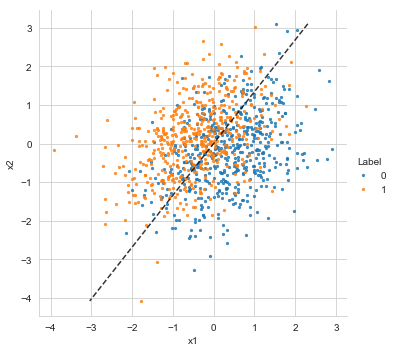
\includegraphics[width=5cm]{./logistic.png} 
\end{center}

$\rightharpoondown$ Relax the Gaussian assumption ? (\alert{logistic model, SVM}).

$\rightharpoondown$ Design  nonlinear classification rules ? (\alert{kernels, neural networks}).

\end{frame}

\begin{frame}{The logistic model}

\begin{itemize}
\item One of the most widely used classification algorithm.

\item Logistic model is the "brother" of the linear model in the context of binary classification 
($\Yc = \{-1, 1\}$).

\item We want to explain the label $Y$ based on $X$, we want to
"regress" $Y$ on $X$.

\item It \structure{models the distribution of $Y|X$}.
For $y\in \{-1, 1\}$
$$
\P\left(  Y = 1 | X =x \right) = \sigma \left( x^T w +b \right)
$$
where $w\in \R^d$ is a vector of model weights and $b\in\R$ is the
intercept, and where $\sigma$ is the \structure{sigmoid} function:
\end{itemize}
\begin{minipage}{0.45\textwidth}
$$
\sigma(z) = \frac{1}{1+e^{-z}}. 
$$
\end{minipage}
\begin{minipage}{0.35\textwidth}
\begin{figure}[H]
\begin{center}
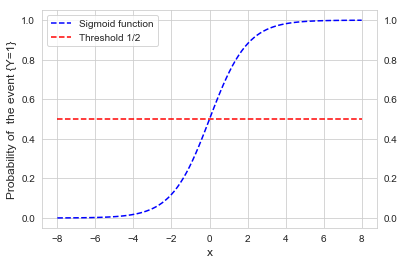
\includegraphics[height=2cm]{./sigmoid}
%\caption{The sigmoid function}
\end{center}
\end{figure}
\end{minipage}
\end{frame}



\begin{frame}{Some comments on the logistic model}
\begin{itemize}
\item The sigmoid choice really is a choice. It is a modelling choice.
\item It's a way to map $\R \to [0, 1]$ (we want to model a probability).
\item We could also consider
$$
\P\left(  Y = 1 | X =x \right) = F \left( x^T w +b \right)
$$
for any distribution function $F$. 
\item Another popular choice is the
Gaussian distribution
$$ F(z) = \P(\Nc(0,1) \leq  z),
$$
which leads to another loss called {\color{PineGreen}probit}.
\end{itemize}
\end{frame}

\begin{frame}{The logistic model}

\begin{itemize}
\item In the case of the sigmoid,
one has
\begin{align*}
\P\left(  Y = 1 | X \right) &= \frac{\exp (b+ w^\top X)}{1+ \exp(b+ w^\top X)} = \frac{1}{1+\exp(-(b+ w^\top X)) } \\
\P\left(  Y = - 1 | X \right) &=  \frac{1}{1+\exp(b+ w^\top X) }
\end{align*}

\item However, the sigmoid choice has the following nice interpretation: an easy computation leads to
$$
\log \left( \frac{\P\left(  Y = 1 | X \right)}{\P\left(  Y = -1 | X  \right)} \right) = X^\top w +b.
$$
\item This quantity is called the \structure{log-odd ratio}.
\end{itemize}
\end{frame}

\begin{frame}{The logistic model}

\begin{itemize}
\item Therefore, this model makes the assumption that \structure{(the logit transformation of) the probability $p(X)=\P\left(  Y = 1 | X \right)$  is linear}:
$$
\mathrm{logit} (p(X)) := \log\left( \frac{p(X)}{1-p(X)} \right) = X^\top w + b.
$$
\pause
\item Note that 
\begin{block}{}
$$
\P\left(  Y = 1 | X \right) \geq \P\left(  Y = -1 | X \right)
$$
\underline{if and only if}
$$
X^\top w + b \geq 0.
$$
\end{block}
\pause
This is a \structure{linear classification rule}, linear w.r.t.\ the considered features $x$!
\end{itemize}
\end{frame}


\begin{frame}{The logistic "regression"}
\begin{theorem}
%	Let us consider that we have $C=2$ classes.
%	Then, under assumption that logit-transformation is linear, we have
%	$$
%		(b^\star, w^\star) \in \argmin_{(b, w)\in\R^\times\R^d} \E \left[\log\left( 1 + \exp(-Y(b + w^\top X)) \right) \right].
%	$$
%	Let
%	$$
%		(\bar b, \bar w) \in \argmin_{(b, w)\in\R^\times\R^d} \E \left[\log\left( 1 + \exp(-Y(b + w^\top X)) \right) \right].
%	$$
%	Then, under assumption that the logit-transformation is linear,
%	a Bayes classifier is
%	$$
%		g^\star \colon x \in \R^d \mapsto
%		\left\{ \begin{array}{ll}
%			+1 & \text{if } \bar b + \bar w ^\top x > 0 \\
%			-1 & \text{otherwise}.
%		\end{array} \right.
%	$$
	Let us consider that $C=2$ and that the logit-transformation is linear with parameters $(b^\star, w^\star)$.
	Let $f^\star \colon x \in \R^d \mapsto b^\star + (w^\star) ^\top x$.

	Then $f^\star$ is a minimizer of the risk functional
	$f \mapsto \E \left[\log\left( 1 + \exp(-Yf(X)) \right) \right]$ over all affine functions and
	$$
		g^\star \colon x \in \R^d \mapsto
		\left\{ \begin{array}{ll}
			+1 & \text{if } f^\star(x) > 0 \\
			-1 & \text{otherwise}
		\end{array} \right.
	$$
	is a Bayes classifier.
\end{theorem}
\end{frame}

\begin{frame}[allowframebreaks]{Proof}

	First, let us remark that $g^\star$, as previously defined, is a Bayes classifier, since $f^\star(x) > 0$ if and only if $\P(Y=+1 | X=x) > \P(Y=-1 | X=x)$.

	Second, without loss of generality, we consider that $b$ vanishes and we denote $\ell \colon (x, y, w) \mapsto \log\left( 1 + \exp(-y w^\top x) \right)$.
	Then, $\forall (x, y) \in \R^d \times \R$,
	$$
		\nabla_{w}{\ell}(x, y, w)
		= - \frac{y}{1+\exp(y w^\top x)} x
		= - \frac{y \exp(-y w^\top x)}{1+\exp(-y w^\top x)} x.
	$$
	Thus, since $\nabla_{w}{\ell}$ is Lebesgue-measurable, we can switch derivative and integral, leading to:
	\begin{align*}
		\nabla_w & {\E(\ell(X, Y, w)|X)}\\
		&= \P(Y=+1 | X) \nabla_w{\psi}(X, 1, w) + \P(Y=-1 | X) \nabla_w{\psi}(X, -1, w) \\
		&= - \frac{\exp((w^\star)^\top x)}{1+\exp((w^\star)^\top x)} \frac{1}{1+\exp(w^\top X)} X \\
		&\quad +
		\frac{1}{1+\exp((w^\star)^\top x)} \frac{\exp(w^\top X)}{1+\exp(w^\top X)} X.
	\end{align*}
	Thus, $\nabla_{w}{\E(\ell(X, Y, w^\star)|X)} = 0$ and $\nabla_{w}{\E(\ell(X, Y, w^\star))} = 0$.
	Since $\ell$ is convex in $w$, this proves that $w^\star$ is a minimizer of $\E(\ell(X, Y, \cdot))$.
\end{frame}

\begin{frame}{Estimation of $w$ and $b$}

\begin{itemize}
\item We have a model for the conditional law of $Y$ given $X$.
\item Data $(X_i , Y_i)$ is assumed i.i.d with the same distribution as $(X,Y)$.
\item Compute estimators $\hat{w}$ and $\hat{b}$ by maximum likelihood estimation
\item Or equivalently, minimize the minus log-likelihood.
\item  More generally, when a model is used
\begin{center}
Goodness-of-fit = -log likelihood
\end{center}
log is used mainly since averages are easier to study (and compute) than products.
\end{itemize}  
\end{frame}

\begin{frame}{Logistic regression - likelihood function}

$\rightharpoondown$   $\{(X_i,Y_i)\}_{1\leqslant i\leqslant n}$ are \alert{i.i.d. with the same distribution as $(X,Y)$}.

{\bf\structure{Likelihood}}

\begin{align*}
 \prod_{i=1}^n \P(Y_i | X_i) &= \prod_{i=1}^n \sigma(\langle w,X_i \rangle + b)^{Y_i} \big(1 - 
\sigma(\langle w,X_i \rangle + b) \big)^{1 - Y_i}\,, \\
& = \prod_{i=1}^n \sigma(\langle w,x_i \rangle + b)^{Y_i} 
\sigma(-\langle w,X_i \rangle - b)^{1 - Y_i}
\end{align*}
\smallskip

and the \alert{normalized negative loglikelihood} is 
\smallskip

\begin{equation*}
f(w,b) = \frac{1}{n}\sum_{i=1}^n \ell(Y_i, \langle w,X_i \rangle + b)\,.
\end{equation*}
\end{frame}


\begin{frame}{Logistic regression - likelihood function}
		
Compute $\hat w_n$ and $\hat b_n$ as follows:

\begin{align*}
(\hat w_n, \hat b_n) \in \argmin_{w \in \R^d, b \in \R}
\frac 1n \sum_{i=1}^n\left(-Y_i (X_i^\top w+ b) +  \log(1+ e^{X_i^\top w + b})\right)\,.
\end{align*}

\vspace{.3cm}

$\rightharpoondown$ It is an \textbf{average of losses}, one for each sample point.

$\rightharpoondown$ It is a \alert{convex and smooth problem}.


\medskip

Using the \textbf{\alert{logistic loss}} function
\smallskip 

\begin{equation*}
\ell: (y, y') \mapsto \log(1 + e^{-y y'}) 
\end{equation*}

yields

\begin{equation*}
(\hat w_n, \hat b_n) \in \argmin_{w \in \R^d, b \in \R}
\frac 1n \sum_{i=1}^n \ell(Y_i, \langle w,X_i \rangle + b)\,.
\end{equation*}
\end{frame}


%\begin{frame}{The logistic "regression"}
%By introducing the logistic loss function
%$$
%\ell (y , y') = \log (1+e^{-yy'} ),
%$$
%then
%$$
%\hat{w}, \hat{b} \in \argmin_{w\in \R^d \atop b \in \R} \frac{1}{n} \sum_{i=1}^n \ell (y_i , x_i^T w+b).
%$$
%
%\begin{itemize}
%\item It is a convex and smooth problem
%\item Many ways to find an approximate minimizer 
%\item Efficient convex optimization algorithms (more on that later)
%\end{itemize}
%\end{frame}

\begin{frame}{But...}
\begin{remark}
However, if there exists a separating hyperplane for $(X_i,Y_i)_{1\leq i \leq n}$ i.e.\ if there exists $(b_0,w_0)$ such that
$$
\forall i=1,\hdots , n , \qquad Y_i (w_0^T X_i +b_0) >0,
$$
then there is no minimizer of the negative log-likelihood! 
\end{remark}
\end{frame}

\begin{frame}{Summary: LDA/QDA/Logistic reg}


 \textbf{Logistic regression} directly models the parameter of the distribution of \structure{$Y$ given $X$}.

\begin{itemize}
\item The \structure{logit transformation of the probability} $p(X)=\P\left(  Y = 1 | X \right)$  is \alert{linear}:
$$
\mathrm{logit} (p(X)) := \log\left( \frac{p(X)}{1-p(X)} \right) = X^\top w + b.
$$
\end{itemize}

\textbf{Linear discriminant analysis} do the opposite. 

\begin{itemize}
\item It models the distributions of \structure{$X$ given $Y = j$} for $j = 1,...,M$ by Gaussian distributions $f_j(x)$,
\item  The posterior distribution of $Y$ given $X$ can be computed with Bayes formula:
$$
\P \left( Y =j | X \right) = \frac{\pi_j f_j(X) }{\sum_\ell^M \pi_\ell f_\ell(X)},
$$
with $\pi_j = \P(Y=j)$.
\end{itemize}

\end{frame}

\begin{frame}{Summary: LDA/QDA/Logistic reg}

\begin{itemize}
\item Classification rule: we choose the group which maximizes these probabilities
$\hat{g}(X)=k$ if and only if $\P(Y=k|X)\geq \P(Y=j|X), \forall j \neq k$.
\item Boundary between 2 groups: set of points x such that 
$$\P (Y =k|X )=\P(Y =j|X )$$
i.e.\
\begin{align*}
0 &= \log\left(\frac{\P (Y =k|X)}{\P(Y =j|X)} \right) =  \log\frac{f_k(X)}{f_j(X)}+ 	\log\frac{\pi_k}{\pi_j} \\
&= \log\frac{\pi_k}{\pi_j} + \frac{1}{2} (\mu_k + \mu_j)^T \Sigma^{-1} (\mu_k - \mu_j) + X^\top \Sigma^{-1} (\mu_k - \mu_j)
\end{align*}
which is \alert{linear} in $x$!
\end{itemize}

\end{frame}

%\begin{frame}
%
%\begin{figure}
%\begin{center}
%\includegraphics[width=\textwidth]{notes/img/lda_qda_log}
%\end{center}
%\caption{Comparison between LDA, QDA and logistic regression}
%\end{figure}
%
%\end{frame}


\section{Linear Support Vector Machine (SVM)}


\begin{frame}{Linear Support Vector Machine (SVM)}
 \begin{itemize}
    \item Binary classification problem
    \item We observe a training dataset of pairs $(x_i, y_i)$ for $i=1, \ldots, n$
    \item Features $x_i \in \R^d$ and labels $y_i \in \{ -1, 1 \}$
    \item Aim is to learn a classification rule that \textbf{generalizes} well
    \item Given a features vector $x \in \R^d$, we want to predict the label $y$ 
    \item Without \textbf{overfitting}
  \end{itemize}
\end{frame}

\subsection{Preliminary}

\begin{frame}{Linear classification}
  Why?
  \begin{itemize}
    \item It's simple!
    \item On very large datasets ($n$ is large, say $n \geq 10^7$), no other choice (training complexity)
    \item Big data paradigm: lots of data $\Rightarrow$ simple methods are enough
  \end{itemize}

  % What is a linear classifier
  % \begin{itemize}
  % \item Using training data $(x_1, y_1), \ldots, (x_n, y_n)$,
  %   construct a decision rule $f$ that predict the label $\hat y$ of a
  %   new data point $x$    
  % \item We saw that the logistic classifier is linear:
  %   where $\sign z = 1$ if $z > 0$ and $\sign z = -1$ if $z < 0$, and
  %   where $\hat \beta \in \R^d$ and $\hat b \in \R$ is the intercept
  % \item The aim of linear classification is to find $\hat \theta$ and
  %   $\hat b$ using the training data
  % \end{itemize}

  \medskip


  
  \begin{block}{A linear classifier}
  
  \begin{tabular}[htbp]{cc}    
    \begin{minipage}[htbp]{.5\linewidth}
      \vspace{0.2cm}
      \begin{center}
  				\includegraphics[width=5cm]{../../../ISUP2018/notes/img/SVM/lda_binary}
      \end{center}
    \end{minipage}
    &
    \begin{minipage}[htbp]{.5\linewidth}
      Learn $\hat w \in \R^d$ and $\hat b$ s.t.\       
      \begin{equation*}
        \hat y = \sign(\langle {x, \hat w} \rangle + \hat b)
      \end{equation*}
      is a good classifier
    \end{minipage}
	\end{tabular}
  \end{block}
\end{frame}


%\subsection{Linearly separable data}



  \begin{frame}{Preliminary definitions}
  
  \begin{exampleblock}{}
A dataset is {\color{Vert} linearly separable} if we can find an hyperplane $H$ that puts 
\begin{itemize}
  \item Points $x_i \in \R^d$ such that $y_i = 1$ on one side of the hyperplane
  \item Points $x_i \in \R^d$ such that $y_i = -1$ on the other
  \item $H$ do not pass through a point $x_i$
\end{itemize}
\end{exampleblock}

\begin{center}
  \includegraphics[width=0.5\textwidth]{../../../ISUP2018/notes/img/SVM/hyperplane.png}
\end{center}
\end{frame}



\begin{frame}{Preliminary definitions}
\begin{exampleblock}{}
  An {\color{Vert}hyperplane }
  \begin{equation*}
      H = \{ x \in \R^d : w^T x + b = 0 \}
  \end{equation*}
  is a translation of a set of vectors orthogonal to $w$
  \begin{itemize}
    \item $w \in \R^d$ is a non-zero vector normal to the hyperplane
    \item $b \in \R$ is a scalar 
  \end{itemize}
 \end{exampleblock}
  
  
    Definition of $H$ is invariant by multiplication of $w$ and $b$ by a non-zero scalar
\end{frame}






\begin{frame}{Canonical hyperplane}

  If $H$ do not pass through any sample point $x_i$, we can scale $w$ and $b$ so that
  \begin{equation*}
    \min_{(x, y) \in D_n} |w^T x + b| = 1
  \end{equation*}
    For such $w$ and $b$, we call $H$ the {\color{Vert}canonical} hyperplane
    
    
  \begin{figure}
  \begin{center}
    \includegraphics[width=0.5\textwidth]{../../../ISUP2018/notes/img/SVM/canonical_hyperplane.png}
    \caption{The marginal hyperplanes are the hyperplanes parallel to the separating hyperplane and passing through the closest points on the negative or positive sides.}
  \end{center}
  \end{figure}


\end{frame}


\begin{frame}{The margin}
  The distance of any point $x' \in \R^d$ to $H$ is given by
  \begin{equation*}
    \frac{|\langle {w, x'} \rangle  + b|}{\norm{w}}
  \end{equation*}

\begin{exampleblock}{}
  So, if $H$ is a canonical hyperplane, its {\color{Vert}margin} is given by
  \begin{equation*}
    \min_{(x, y) \in D_n}   \frac{|w^T x + b|}{\norm{w}} 
    = \frac{1}{\norm{w}}.
  \end{equation*}
 \end{exampleblock}

  \begin{center}
    \includegraphics[width=6cm]{../../../ISUP2018/notes/img/SVM/margin}
  \end{center}

\end{frame}



\begin{frame}{Summary}
If $\Dc_n$ is strictly \structure{linearly separable}, we can find a \structure{canonical separating hyperplane} 
\begin{equation*}
  H = \{ x \in \R^d : w^T x + b = 0 \}.
\end{equation*}
that satisfies
\begin{equation*}
  |\langle {w, x_i} \rangle  + b| \geq 1 \; \text{ for any } \; i=1, \ldots, n,
\end{equation*}
which entails that a point $x_i$ is correctly classified if
\begin{equation*}
  y_i (\langle {x_i, w} \rangle  + b) \geq 1.
\end{equation*}
The \structure{margin} of $H$ is equal to $1 / \norm{w}$.
\end{frame}




\subsection{Linear SVM: separable case}
\begin{frame}{Linear SVM: separable case}

\begin{block}{Maximum margin problem}
A way of classifying $\Dc_n$ with maximum margin is to solve the following problem:
\begin{align*}
  &\min_{w \in \R^d, b \in \R} \frac 12 \norm{w}_2^2 \\
  &\text{ subject to } \;\;  y_i (\langle {x_i, w} \rangle  + b) \geq 1 \; \text{ for all } 
  \;i=1, \ldots, n
\end{align*}
\end{block}

\medskip

Note that:
\begin{itemize}
  \item This problem admits a \alert{unique} solution
  \item It is a ``quadratic programming'' problem, which is easy to solve numerically
  \item Dedicated optimization algorithms can solve this on a large scale very efficiently
\end{itemize}
\end{frame}


\subsection{Lagrangian duality}
\begin{frame}{Tools from constrained convex optimization}

  \begin{itemize}
    \item Consider a constrained optimization problem
  \begin{align*}
    \min_{x \in \R^d} & \quad f(x) \\
    \text{ subject to } \;\; & h_i(x) = 0 \; \text{ for all } 
    \;i=1, \ldots, p \\
   	 & g_j(x) \leq 0 \; \text{ for all } 
    \;j=1, \ldots, q
  \end{align*}
  where $f, h_1, \hdots h_p, g_1, \ldots, g_q : \R^d \rightarrow \R$
  \item Denote $P^\star = f(x^\star)$ the minimum of the \textbf{primal} pb
    \end{itemize}
    
    \begin{block}{Lagrangian}
   The associated \textbf{Lagrangian} is the function given on $\R^d \times \R^p\times \R_+^q$ by
  \begin{equation*}
    L(x, \lambda, \mu) = f(x) + \sum_{i=1}^p \lambda_i h_i(x) + \sum_{j=1}^q \mu_j g_j(x)
  \end{equation*}
  \end{block}
    $\lambda = (\lambda_1, \ldots, \lambda_q) \in \R^p$,   $\mu = (\mu_1, \ldots, \mu_q) \in \R_{\alert{+}}^q$ are called \textbf{Lagrange} or \textbf{dual} variables.

\end{frame}


\begin{frame}[allowframebreaks]

\begin{block}{ The {Lagrange dual} function }
    \begin{align*}
      D(\lambda, \mu) &:= \inf_{x \in \R^d} L(x, \lambda, \mu) \\
      &= \inf_{x \in \R^d} 
      \left( f(x) + \sum_{i=1}^p \lambda_i h_i(x) + \sum_{j=1}^q \mu_j g_j(x) \right)
    \end{align*}
    for $(\lambda, \mu) \in \R^p \times \R_+^q$
\end{block}
  \begin{itemize}
    \item $D$ is always concave, as the infimum of linear functions
    \item Denote $D^\star := D(\lambda^\star, \mu^\star) = \max_{\lambda\atop \mu \geq 0} D(\lambda, \mu)$ the optimal value of the dual. It is a convex problem (maximum of a concave function)
    \item For any \textbf{feasible} $x$ and any $(\lambda, \mu) \in \R^p \times \R_+^q$ we have $D(\lambda, \mu) \leq f(x)$, hence
    \begin{block}{Weak duality}
    \begin{equation*}
      D^\star \leq P^\star
    \end{equation*}
    \end{block}
    This  \structure{always} holds!
    \item Something that \alert{does not} always holds is
    \begin{block}{Strong duality}
    \begin{equation*}
      D^\star = P^\star
    \end{equation*}
    \end{block}
  \end{itemize}
\end{frame}


\begin{frame}{Lagrangian duality}
  \alert{Strong duality} holds under 
  \begin{itemize}
  \item \structure{convexity} of the problem 
  \item \structure{constraint qualifications} 
  \end{itemize}

  \medskip
  A simple way to have constraint qualification (sufficient but not necessary)
    \begin{block}{Slater's conditions}
    There is some strictly feasible point $x \in \R^d$ such that
    \begin{align*}
      h_i(x) = 0 &\quad \text{for all } i=1, \ldots, p \\
      g_j(x) < 0 &\quad \text{for all } j=1, \ldots, q
    \end{align*}
    \end{block}
\end{frame}

\begin{frame}{Karush-Kuhn-Tucker (KKT) conditions}

  \begin{enumerate}[(i)]
    \item Assume that $f, g_1, \ldots, g_q$ are \textbf{differentiable}, \textbf{convex}, 
    \item $h_1,\hdots h_p$ are \textbf{affine} functions
    \item Assume Slater's condition
    \end{enumerate}
    \begin{block}{NSC for optimality}
    Under (i), (ii), (iii), 
    
    $x^\star \in \R^d$ is a solution of the primal problem \underline{if and only if} there is $(\lambda^\star, \mu^\star \in \R^p\times\R_+^q$ such that
    \begin{align*}
      \nabla_x L(x^\star, \lambda^\star, \mu^\star) &= \nabla f(x^\star) 
      + \sum_{i=1}^n \lambda_i^\star \nabla h_i(x^\star) 
      + \sum_{j=1}^n \mu_j^\star \nabla g_j(x^\star) = 0 \\
      h_i(x^\star) &= 0 \quad \text{ for any } i=1, \ldots, p \\
      g_j(x^\star) &\leq 0 \quad \text{ for any } j=1, \ldots, q \\
      \mu_j^\star g_j(x^\star) &= 0 \quad \text{ for any } j=1, \ldots, q \\
    \end{align*}
    \end{block}
\end{frame}



\begin{frame}{}
    \begin{itemize}
    \item These are known as the \alert{KKT conditions}
    \item The last one is called \structure{complementary slackness}
  \end{itemize}
  \begin{block}{Take-home message: Lagrangian duality}
 If
  \begin{itemize}
    \item[$\circ$] primal problem is \textbf{convex} and
    \item[$\circ$] constraint functions satisfy the \textbf{Slater}'s conditions
  \end{itemize}
  then
  \begin{itemize}
     \item \textbf{strong duality} holds. 
   \end{itemize} 

  \bigskip
  If in addition we have that
  \begin{itemize}
    \item[$\circ$] functions $f, g_1, \ldots, g_n$ are \textbf{differentiable}
  \end{itemize}
  then
  \begin{itemize}
    \item KKT conditions are \textbf{necessary and sufficient} for optimality
  \end{itemize}
  \end{block}
\end{frame}

\begin{frame}
\textbf{Exercise} \\
Now that you know about the Lagrangian duality, you can prove that the distance of a point to the canonical hyperplane is well given by the formula on Slide 10!
\end{frame}



\subsection{Back to the Linear SVM} 

\begin{frame}{Back to the linear SVM}

The problem has the form
\begin{block}{}
\begin{align*}
  &\min_{w \in \R^d, b \in \R} f(w) \\
  &\text{ subject to } \;\;  g_i(w, b) \leq 0 \; \text{ for all } 
  \;i=1, \ldots, n
\end{align*}
\end{block}
where
\begin{itemize}
  \item $f(w) = \frac 12 \norm{w}_2^2$ is \textbf{strongly convex}, since
  \begin{equation*}
      \nabla^2 f(w) = I_d \succ 0    
  \end{equation*}
  \item Constraints are $g_i(w, b) \leq 0$ with \textbf{affine} functions
  \begin{equation*}
    g_i(w, b) =  1 - y_i (\langle {x_i, w} \rangle  + b)
  \end{equation*}
  so that the constraints are \textbf{qualified}
\end{itemize}
\end{frame}

\begin{frame}{Back to the linear SVM}




KKT theorem 
  \begin{itemize}
    \item Leads to crucial properties on the SVM
    \item Allows to obtain the dual formulation of the problem
  \end{itemize}

  \bigskip
  \begin{block}{Lagragian}
  \begin{itemize}
    \item Introduce dual variables \structure{$\mu_i \geq 0$} for $i=1, \ldots, n$ corresponding to the constraints $g_i(w, b) \leq 0$
    \item For $w \in \R^d$, $b \in \R$ and $\mu = (\mu_1, \ldots \mu_n) \in \R_+^n$, define the Lagrangian
    \begin{equation*}
      L(w, b, \mu) = \frac 12 \norm{w}_2^2 + \sum_{i=1}^n \mu_i \big(1 - y_i( \langle {w, x_i} \rangle  + b) \big)
    \end{equation*}
  \end{itemize}
  \end{block}
  
  \end{frame}



\begin{frame}{KKT and linear SVM}
  \begin{equation*}
    L(w, b, \mu) = \frac 12 \norm{w}_2^2 + \sum_{i=1}^n \mu_i \big(1 - y_i( \langle {w, x_i} \rangle  + b) \big)
  \end{equation*}

  \begin{block}{KKT conditions}
  
    Set the gradient to zero
    \begin{align*}
      \nabla_w L(w, b, \mu) &= w - \sum_{i=1}^n \mu_i y_i x_i = 0 \quad \text{namely} \quad w = \sum_{i=1}^n \mu_i y_i x_i \\
      \nabla_b L(w, b, \mu) &= -\sum_{i=1}^n \mu_i y_i = 0 \quad \text{namely} \quad \sum_{i=1}^n \mu_i y_i =0
    \end{align*}
    Write the complementary slackness condition: $\forall i=1,\hdots,n$
    \begin{equation*}
      \mu_i \big(1 - y_i(\langle {w, x_i} \rangle + b) \big) = 0 \quad \text{namely} \quad \mu_i = 0 \; \text{ or } \; y_i(\langle {w, x_i} \rangle  + b) = 1
    \end{equation*} 
    \end{block}
\end{frame}


    



\begin{frame}{SVM that's the name}
At the optimum,
\begin{itemize}
  \item There are \textbf{dual} variables $\mu_i \geq 0$ such that the \textbf{primal} solution $(w, b)$ satisfies
\begin{equation*}
    w = \sum_{i=1}^n \mu_i y_i x_i
\end{equation*}
\item We have that
  \begin{equation*}
      \mu_i \neq 0 \quad \text{iff} \quad y_i (\langle {w, x_i} \rangle  + b) = 1
  \end{equation*}
\end{itemize}
\pause 
This means that
\begin{itemize}
    \item $w$ writes as a linear combination of the features vectors $x_i$ that belong to the marginal hyperplanes $\{ x \in \R^d : w^T x + b = \pm 1 \}$
\item These vectors $x_i$ are called \structure{support vectors}
\end{itemize}


\medskip
The support vectors fully define the maximum-margin hyperplane, hence the name 
\textbf{\alert{Support Vector Machine}}
\end{frame}

\begin{frame}{SVM that's the name}
\begin{figure}
\begin{center}
\includegraphics[height=5cm]{img/support_vectors}
\end{center}
\end{figure}

\end{frame}



  \begin{frame}[allowframebreaks]{Dual optimization problem}
Under \structure{strong duality}, primal and dual problems are strongly related, and one can be used to solve the other.


\begin{itemize}
\item  Recall that the Lagrangian is
  \begin{equation*}
    L(w, b, \mu) = \frac 12 \norm{w}_2^2 + \sum_{i=1}^n \mu_i \big(1 - y_i( \langle {w, x_i} \rangle  + b) \big)
  \end{equation*}  
\item   Plug $w = \sum_{i=1}^n \mu_i y_i x_i$ in it to obtain
  \begin{align*}
    L(w, b, \mu) &= \frac 12 \Big\| \sum_{i=1}^n \mu_i y_i x_i \Big\|_2^2 
    + \sum_{i=1}^n \mu_i - b \sum_{i=1}^n \mu_i y_i \\
       &\quad - \sum_{i, j=1}^n \mu_i \mu_j y_i y_j \langle {x_i, x_j} \rangle 
  \end{align*}
 \item  Recalling that $\sum_{i=1}^n \mu_i y_i = 0$ and doing some algebra we arrive at the dual formulation

\begin{block}{Dual formulation}

  \begin{align*}
      &\max_{\mu \in \R^n} \quad \quad \sum_{i=1}^n \mu_i - \frac 12 \sum_{i, j=1}^n \mu_i \mu_j y_i y_j \langle {x_i, x_j} \rangle  \\
    &\text{subject to} \quad \mu_i \geq 0 \; \text{ and } \; 
    \sum_{i=1}^n \mu_i y_i  = 0 \; \text{ for all } \; i=1, \ldots, n
  \end{align*}
  \end{block}
  \end{itemize}

\end{frame}

\begin{frame}{Comments}

  \begin{itemize}
    \item As in the primal formulation, it is again a quadratic programming problem
    \item At optimum, we have (using KKT conditions) that the decision function is expressed using the dual variables as
    \begin{equation*}
      x \mapsto \mathop{sign}(w^T x + b) = \mathop{sign}\Big(  \sum_{i=1}^n \mu_i y_i 
      \langle {x, x_i} \rangle  + b \Big)
    \end{equation*}
    \item The intercept $b$ can be expressed for any support vector $x_i$ as
    \begin{equation*}
      b = y_i -  \sum_{j=1}^n \mu_j y_j \langle {x_i, x_j} \rangle 
    \end{equation*}
    
  \end{itemize}
\end{frame}



\begin{frame}{About the margin}
This allows to write the margin as a function of the dual variables
\begin{itemize}
  \item Multiplying the last equality by $\mu_i y_i$ and summing entails
    \begin{equation*}
      \sum_{i=1}^n \mu_i y_i b =  \sum_{i=1}^n \mu_i y_i^2 - \sum_{i, j=1}^n \mu_i \mu_j y_i y_j \langle {x_i, x_j} \rangle 
    \end{equation*}
    \pause
  \item Namely recalling that at optimum $\sum_{i=1}^n \mu_i y_i = 0$ and $w = \sum_{i=1}^n \mu_i y_i x_i$ we get
  \begin{align*}
    0 &= \sum_{i=1}^n \mu_i = \norm{w}_2^2, \quad \text{ namely } \\
      \text{margin} &= \frac{1}{\norm{w}_2^2} = \frac{1}{\sum_{i=1}^n \mu_i} 
    = \frac{1}{\norm{\mu}_1}
  \end{align*}
	\pause 
  \item Okay, this is a nice theory, but...
\end{itemize}
\end{frame}


\begin{frame}
  Have you ever seen a dataset that looks like this?
  
  \begin{center}
    \includegraphics[width=0.4\textwidth]{../../../ISUP2018/notes/img/SVM/hyperplane}
  \end{center}
  
  Datasets are generally \alert{not} linearly separable!

\end{frame}

 \begin{frame}{Relaxation for the non-separable case}
  Keep cool and \textbf{relax} !

  \bigskip
  Replace the constraints
  \begin{equation*}
    y_i (\langle {w, x_i} \rangle  + b) \geq 1 \;\; \text{ for all } \;\;
    i=1, \ldots, n,
  \end{equation*}
  \pause
  that are too strong, by the \textbf{relaxed} ones
  \begin{equation*}
    y_i (\langle {w, x_i} \rangle  + b) \geq 1 - s_i \;\; \text{ for all } \;\;
    i=1, \ldots, n,
  \end{equation*}
  for \textbf{\structure{slack variables}} $s_1, \ldots, s_n \geq 0$
\end{frame}







\subsection{Linear SVM: non-separable case}

\begin{frame}{Linear SVM: non-separable case}
Relax, but keep the slacks $s_i$ as small as possible (goodness-of-fit)

Replace the original problem
\begin{align*}
  &\min_{w \in \R^d, b \in \R} \frac 12 \norm{w}_2^2 \\
  &\text{ subject to } \;\;  y_i (\langle {x_i, w} \rangle  + b) \geq 1 \; \text{ for all } 
  \;i=1, \ldots, n
\end{align*}
by the relaxed one using slack variables
\begin{block}{}
\begin{align*}
  &\min_{w \in \R^d, b \in \R, s \in \R^n} \frac 12 \norm{w}_2^2 
  + C \sum_{i=1}^n s_i \\
  &\text{ subject to } \;\;  y_i (\langle {x_i, w} \rangle  + b) \geq 1 - s_i \; 
  \text{ and } \; s_i \geq 0 \; \forall  \;i=1, \ldots, n
\end{align*}
\end{block}
where $C > 0$ is the ``goodness-of-fit strength''
\end{frame}


\begin{frame}{}
  \begin{itemize}
    \item The slack $s_i \geq 0$ measures the the distance by which $x_i$ violates the desired inequality $y_i (\langle {x_i, w} \rangle  + b) \geq 1$ 
   \pause
    \item A vector $x_i$ with $0 < y_i (\langle {x_i, w} \rangle  + b) < 1$ is correctly classified but is an outlier, since $s_i > 0$
    \pause
    \item If we omit outliers, training data is correctly classified by the hyperplane $\{ x \in \R^d : \langle {x, w} \rangle  + b = 0 \}$ with a margin $1 / \norm{w}_2^2$
    \pause
    \item The margin $1 / \norm{w}_2^2$ is called a \textbf{\structure{soft-margin}} (in the non-separable case), while it is a \textbf{\structure{hard-margin}} in the separable case
  \end{itemize}

  \begin{center}
    \includegraphics[width=0.5\textwidth]{../../../ISUP2018/notes/img/SVM/soft_hard_margin}  
  \end{center}
 \end{frame}   




\begin{frame}{Linear SVM: non-separable case}

So, we arrived at:
\begin{block}{Relaxed margin problem}
\begin{align*}
  &\min_{w \in \R^d, b \in \R, s \in \R^n} \frac 12 \norm{w}_2^2 
  + C \sum_{i=1}^n s_i \\
  &\text{ subject to } \;\;  y_i (\langle {x_i, w} \rangle + b) \geq 1 - s_i \; 
  \text{ and } \; s_i \geq 0 \; \text{ for all }  \;i=1, \ldots, n
\end{align*}
\end{block}

Once again:
\begin{itemize}
  \item This problem admits a \textbf{unique} solution
  \item It is a quadratic programming problem
\end{itemize}

\medskip
The constant $C > 0$ is chosen using $V$-fold cross-valiation
\end{frame}



\begin{frame}{Linear SVM: non-separable case}
  \begin{block}{Lagrangian}
  \begin{align*}
    L(w, b, s, \mu, \beta) &= \frac 12 \norm{w}_2^2 + C \sum_{i=1}^n 
    s_i \\ 
    & \quad + \sum_{i=1}^n \mu_i \big(1 - s_i - y_i( \langle {w, x_i} \rangle  + b) \big) 
    - \sum_{i=1}^n \beta_i s_i
  \end{align*}
  with $\mu_i\geq 0$ and $\beta_i \geq 0$.
  \end{block}
  
  At optimum, let's again:
  \begin{itemize}
    \item set the gradients $\nabla_w$, $\nabla_b$ and $\nabla_s$ to zero
    \item write the complementary conditions
  \end{itemize}
\end{frame}


\begin{frame}{Linear SVM: non-separable case}
    \begin{align*}
      \nabla_w L(w, b, s, \mu, \beta) &= w - \sum_{i=1}^n \mu_i y_i x_i = 0 \quad \text{i.e.} \quad w = \sum_{i=1}^n \mu_i y_i x_i \\
      \nabla_b L(w, b, s, \mu, \beta) &= -\sum_{i=1}^n \mu_i y_i = 0 \quad \text{i.e.} \quad \sum_{i=1}^n \mu_i y_i = 0 \\
      \nabla_s L(w, b, s, \mu, \beta) &= C - \mu_i - \beta_i = 0 \quad \text{i.e.} \quad \mu_i + \beta_i = C
    \end{align*}
    and the complementary condition
    \begin{equation*}
      \mu_i \big(1 - s_i - y_i(\langle {w, x_i} \rangle  + b) \big) = 0 \; \text{i.e.} \; \mu_i = 0 \; \text{ or } \; y_i(\langle {w, x_i} \rangle + b) = 1 - s_i
    \end{equation*}
    \begin{equation*}
      \beta_i s_i = 0 \quad \text{ i.e. } \quad \beta_i = 0 \; \text{ or } \; s_i = 0
    \end{equation*}
    for all $i=1, \ldots, n$
\end{frame}


\begin{frame}{Linear SVM: non-separable case}
  This means that
  \begin{itemize}
    \item $w = \sum_{i=1}^n \mu_i y_i x_i$
    \pause
    \item If $\mu_i \neq 0$ we say that $x_i$ is a \structure{support vector} and in this case $y_i(\langle {w, x_i} \rangle  + b) = 1 - s_i$
    \begin{itemize}
      \item If $s_i = 0$ then $x_i$ belongs to a margin hyperplane
      \item If $s_i \neq 0$ then $x_i$ is an outlier and $\beta_i = 0$ and then $\mu_i = C$
    \end{itemize}
  \end{itemize}
  \pause 
  \begin{alertblock}{}
  Support vectors either belong to a marginal hyperplane, or are outliers with $\mu_i = C$
  \end{alertblock}
  \pause
  \begin{figure}
 	\begin{center}
 		\includegraphics[height=4cm]{img/soft_support_vectors}
	\end{center} 	 
  \end{figure}
\end{frame}


\begin{frame}{To the dual problem...}
  \begin{itemize}
    \item Plugging $w = \sum_{i=1}^n \mu_i y_i x_i$ in $L(w, b, s, 
    \mu, \beta)$ leads to the same formula as before
    \begin{equation*}
      \sum_{i=1}^n \mu_i - \frac 12 \sum_{i, j=1}^n \mu_i \mu_j y_i 
      y_j \langle {x_i, x_j} \rangle 
    \end{equation*}
    \pause
    \item with the constraints
    \begin{equation*}
      \mu_i \geq 0, \quad \beta_i \geq 0, \quad  
      \sum_{i=1}^n \mu_i y_i  = 0, \quad \mu_i + \beta_i = C
    \end{equation*}
    that can be rewritten for as
    \begin{equation*}
      0 \leq \mu_i \leq C, \quad  
      \sum_{i=1}^n \mu_i y_i  = 0
    \end{equation*}
    for all $i=1, \ldots, n$
  \end{itemize}
  \end{frame}




  \begin{frame}{Dual problem}
  \begin{block}{Dual problem}
  \begin{align*}
      &\max_{\mu \in \R^n} \quad \quad \sum_{i=1}^n \mu_i - \frac 12 \sum_{i, j=1}^n \mu_i \mu_j y_i y_j \langle {x_i, x_j} \rangle \\
    &\text{subject to} \quad 0 \leq \mu_i \leq C \; \text{ and } \; 
    \sum_{i=1}^n \mu_i y_i  = 0 \; \text{ for all } \; i=1, \ldots, n
  \end{align*}
  \end{block}
  
  \begin{itemize}
    \item This is the same problem as before, but with the extra constraint 
    \begin{equation*}
      \mu_i \leq C 
    \end{equation*}
    \item It is again a convex quadratic program
  \end{itemize}
  \end{frame}



\begin{frame}{Linear SVM: non-separable case}
  As in the linearly separable case, the \structure{label} prediction is expressed using the \structure{dual variables}.
  \begin{block}{Labels given by}
  \begin{equation*}
    x \mapsto \mathop{sign}(w^T x + b) = \mathop{sign}\Big(  \sum_{i=1}^n \mu_i y_i 
    \langle {x, x_i} \rangle  + b \Big)
  \end{equation*}
  \end{block}

  \bigskip
  The intercept $b$ can be expressed for a support vector $x_i$ such that $0 < \mu_i < C$ as
  \begin{equation*}
    b = y_i -  \sum_{j=1}^n \mu_j y_j \langle {x_i, x_j} \rangle
  \end{equation*}
\end{frame}



  \begin{frame}{An important remark}

  The dual problem
  \begin{align*}
      &\max_{\mu \in \R^n} \quad \quad \sum_{i=1}^n \mu_i - \frac 12 \sum_{i, j=1}^n \mu_i \mu_j y_i y_j \langle {x_i, x_j}  \rangle \\
    &\text{subject to} \quad 0 \leq \mu_i \leq C \; \text{ and } \; 
    \sum_{i=1}^n \mu_i y_i  = 0 \; \text{ for all } \; i=1, \ldots, n
  \end{align*}
  and the label prediction (using dual variables)
  \begin{equation*}
    x \mapsto \mathop{sign}(w^T x + b) = \mathop{sign}\Big(  \sum_{i=1}^n \mu_i y_i 
    \langle {x, x_i} \rangle  + b \Big)
  \end{equation*}
  depends only on the features $x_i$ via their \textbf{inner products} $\langle {x_i, x_j} \rangle $ !
  \begin{itemize}
    \item This will be particularly important later: \textbf{kernel methods}
  \end{itemize}
\end{frame}



 \begin{frame}{SVM and the hinge loss} 

  Going back to the primal problem
  \begin{align*}
    &\min_{w \in \R^d, b \in \R, s \in \R^n} \frac 12 \norm{w}_2^2 
    + C \sum_{i=1}^n s_i \\
    &\text{ subject to } \;\;  y_i (\langle {x_i, w} \rangle + b) \geq 1 - s_i \; 
    \text{ and } \; s_i \geq 0 \; \text{ for all }  \;i=1, \ldots, n
  \end{align*}
\pause
  \medskip
  We remark that it can be rewritten as follows.
  \begin{block}{Reformulation of the primal problem}
  \begin{equation*}
    \argmin_{w \in \R^d, b \in \R} \frac 12 \norm{w}_2^2 + C \sum_{i=1}^n 
    \max\Big(0, 1 - y_i (\langle {x_i, w} \rangle + b) \Big).
  \end{equation*}
  \end{block}
\end{frame}



 \begin{frame}{SVM and the hinge loss} 
 \begin{exampleblock}{The hinge loss function}
  \begin{equation*}
    \ell(y, y') = \max(0, 1 - y y') = (1 - y y')_+,
  \end{equation*}
  \end{exampleblock}
  the problem can be written as
  \begin{block}{Reformulation of the primal problem}
  \begin{equation*}
    \argmin_{w \in \R^d, b \in \R} \frac 12 \norm{w}_2^2 + C 
    \sum_{i=1}^n \ell(y_i, \langle {x_i, w} \rangle + b).
  \end{equation*}
  \end{block}

  \medskip
  Leads to an alternative understanding of the linear SVM.

\end{frame}


\begin{frame}{SVM and the hinge loss}
  Recall that the natural loss is the $0/1$ one given by
  \begin{equation*}
    \ell_{0/1}(y, z) = \one_{yz \leq 0}.
  \end{equation*}  
  Instead of the Linear SVM, it would be nice to consider
  \begin{equation*}
        \argmin_{w \in \R^d, b \in \R} \frac 12 \norm{w}_2^2 + C \sum_{i=1}^n 
        \one_{y_i (\langle {x_i, w} \rangle  + b) \leq 0},
  \end{equation*}
  but impossible numerically (NP-hard)

  \bigskip
  Hinge loss is a \textbf{convex surrogate} for the $0/1$ loss
\end{frame}




  



\begin{frame}{Conclusion}
  
\structure{\textbf{LDA/QDA}}
\begin{itemize}
\item Model: $X|Y \sim \Nc$
\end{itemize}
  \structure{\textbf{Logistic regression}}
  \begin{itemize}
  \item Logistic regression has a nice probabilistic interpretation
  \item Model $\mathrm{logit}(\P(Y=1|X)$ is linear in $X$
  \item Relies on the choice of the logit link function
  \item[{\color{Red}\ding{55}}] does not work on separable dataset
  \end{itemize}
  
  \bigskip
  \structure{\textbf{SVM}}
  \begin{itemize}
  \item No model, only aims at separating points
  \item[\color{Emerald}\ding{51}] Thought for separable case
  \item[\color{Emerald}\ding{51}] But can be relaxed for the non-separable case
  \end{itemize}
  \end{frame}


%%%%%%%%%%%%%%%%%%%%%%%%%%%%%%%%%%%%%%%%%
%%%%%%%%%%%%%%%%%%%%%%%%%%%%%%%%%%%%%%%%%
%%%%%%%%%%%%%%%%%%%%%%%%%%%%%%%%%%%%%%%%%
%%%%%%%%%%%%    KERNEL  TRICK                   %%%%%%%%%%%%%
%%%%%%%%%%%%%%%%%%%%%%%%%%%%%%%%%%%%%%%%%
%%%%%%%%%%%%%%%%%%%%%%%%%%%%%%%%%%%%%%%%%
%%%%%%%%%%%%%%%%%%%%%%%%%%%%%%%%%%%%%%%%%

%\section{Kernel methods}
%
%
%\begin{frame}{Kernel methods}
%\begin{itemize}
%\item Widely used in machine learning. 
%\item Extend algorithms such as SVMs to define non-linear decision boundaries. 
%\end{itemize}
%\pause
%\begin{block}{Idea}
%\begin{itemize}
%\item to implicitly define an inner product in a high-dimensional space
%\item replacing the original inner product in the input space with positive definite kernels immediately extends algorithms such as SVMs to a linear separation in that high-dimensional space, or, equivalently, to a non-linear separation in the input space
%\end{itemize}
%\end{block}
%\end{frame}
%
%\begin{frame}{When data are not linearly separable? }
%\begin{columns}
%\begin{column}{0.2\textwidth}
%\begin{figure}
%\includegraphics[height=3cm]{img/non_sep_data}
%\end{figure}
%\end{column}
%\pause
%\begin{column}{0.79\textwidth}
%\begin{figure}
%\begin{center}
%\includegraphics[width=0.99\linewidth]{img/kernel_svm.png}
%\end{center}
%\end{figure}
%\end{column}
%\end{columns}
%
%\vspace{2cm}
%
%\tiny{Stolen from \url{http://efavdb.com/svm-classification/}}
%\end{frame}
%
%
%\begin{frame}{When data are not linearly separable}
%\begin{figure}
%\begin{center}
%\includegraphics[width=\textwidth]{img/lifting}
%\end{center}
%\end{figure}
%
%\end{frame}
%
%\begin{frame}{Kernel methods}
%\begin{block}{SVM}
% In practice, linear separation is often not possible.
%\end{block}
%\begin{exampleblock}{Implicit lifting to a higher dimensional space}
%\begin{itemize}
%\item Use more complex functions to separate the two sets
%\item One way: use a non-linear mapping $\varphi$ from the input space $\Xc$ to a higher-dimensional space $\H$, where linear separation is possible
%\end{itemize}
%\end{exampleblock}
%\end{frame}
% 
% \subsection{Motivations}
% 
% \begin{frame}{Ex: polynomial mapping}
% 
% \begin{block}{Polynomial mapping}
% The \textbf{polynomial} mapping $\varphi : \R^2 \rightarrow \R^6$ 
%  for $x = (x_1, x_2) \in \R^2$
%  \begin{equation*}
%    \varphi(x) = (x_1^2, x_2^2, \sqrt{2} x_1 x_2, \sqrt{2} x_1, \sqrt{2} x_2, 1)
%  \end{equation*}
%  solves the XOR (Exclusive OR) classification problem.
%  \end{block}
%  
%  \pause 
%
%
%  XOR : label $y_i$ is blue iff one of the coordinates of $x_i$ equals 1.
%  
%  \end{frame}
%  
%  \begin{frame}
%  \begin{figure}[H]
%  \begin{center}
%    \includegraphics[width=0.5\textwidth]{../../../ISUP2018/notes/img/xor1.png}
%  \end{center}
%  \caption{ XOR problem linearly non-separable in the input space.}
% \end{figure}
%\pause
%  \begin{itemize}
%     \item Blue and red points \structure{cannot be linearly separated} in $\R^2$
%     \pause
%     \item But \structure{they can using the mapping} $\varphi(x) = (x_1^2, x_2^2, \sqrt{2} x_1 x_2, \sqrt{2} x_1, \sqrt{2} x_2, 1)$, using the hyperplane $x_1 x_2 = 0$
%   \end{itemize}
%\end{frame}
%
%\begin{frame}
%
%  \begin{figure}[H]
%  \begin{center}
%    \includegraphics[width=0.95\textwidth]{../../../ISUP2018/notes/img/xor.png}
%  \end{center}
% \end{figure}
% 
% In (b), the hyperplane $x_1 x_2 = 0$ separates blue points and red points.
%
%  This mapping $\varphi$ is call \structure{polynomial mapping of order 2}. 
%  \end{frame}
%
%\begin{frame}{The polynomial mapping}
%
%  Note that for $x, x' \in \R^2$ we have
%  \begin{align*}
%    \langle{\varphi(x), \varphi(x')} \rangle &=
%    %\Bigg\langle
%    \left\langle
%    \begin{bmatrix}
%      x_1^2 \\ x_1^2 \\ x_2^2 \\ \sqrt 2 x_1 x_2 \\ \sqrt{2} x_1 \\ 
%      \sqrt{2} x_2 \\ 1 \\
%    \end{bmatrix},
%    \begin{bmatrix}
%      x_1^2 \\ x_1'^{2} \\ x_2'^{2} \\ \sqrt 2 x_1' x_2' \\ \sqrt{2} x_1' \\ 
%      \sqrt{2} x_2' \\ 1 \\
%    \end{bmatrix} 
%    %\Bigg\rangle \\
%    \right\rangle \\
%    & = (x_1 x_1' + x_2 x_2' + 1)^2 \\
%    & = (\langle {x, x'} \rangle  + 1)^2
%  \end{align*}
%
%\end{frame}
%
%\subsection{Preliminary definitions}
%
%\begin{frame}{Some definitions}
%\begin{definition}[Kernel]
%A function $k :\Xc \times\Xc \to \R$ is called a kernel over $\Xc$.
%\end{definition}
%\pause 
%The idea is to define a kernel $k$ such that  
%$$\forall (x,x') \in \Xc \times \Xc, \qquad 
%k(x,x') = \langle \varphi (x ) , \varphi(x') \rangle_\H.
%$$
%\begin{itemize}
%\item for some mapping $\varphi = \Xc \to \H$ to a Hilbert space $\H$ 
%\item  $\H$ is called a \structure{feature space}
%\end{itemize}
%\pause
%\underline{Interpretation}: $k$ can be interpreted as a similarity measure between elements of the input space $\Xc$ (or the "raw feature" space).
%\end{frame}
%
%\begin{frame}{Good properties of kernels}
%
%\begin{block}{Efficiency:} 
%\begin{itemize}
%\item $k$ is often significantly more efficient to compute than $\varphi$ and an inner product in $\H$. 
%\item in several common examples, the computation of $k(x,x')$ can be achieved in \structure{$O(\dim \Xc)$} while that of $\langle \varphi (x ) , \varphi(x') \rangle_\H$ typically requires $O(\dim(\H))$ work, with $\dim(\H) \gg N$. 
%\item in some cases, $\dim (\H) = \infty$.
%\end{itemize}
%\end{block}
%
%
%\begin{block}{Flexibility:} 
%\begin{itemize}
%\item  \structure{No need to explicitly define or compute a mapping $\varphi$}
%\item The kernel $k$ can be arbitrarily chosen so long as the existence of $\varphi$ is guaranteed, i.e. $k$ satisfies \structure{Mercer's condition}
%\end{itemize}
%\end{block}
%\end{frame}
%
%
%%\begin{frame}{Mercer's theorem}
%%\begin{theorem}[Mercer's theorem]
%%Let $\Xc \subset \R^N$ be a compact set and let $k :\Xc\times \Xc \to \R$ be a continuous and symmetric function. Then, $k$ admits a uniformly convergent expansion of the form
%%$$
%%k(x,x') = \sum_{\ell=0}^\infty a_\ell \varphi_\ell(x) \varphi_\ell(x'),
%%$$
%%with $a_\ell >0$ \underline{iff} for any square integrable function $c\in L^2(\Xc)$, it holds
%%$$
%%\int \int_{\Xc\times \Xc} c(x) c(x') k(x,x') dx dx' \geq 0.
%%$$
%%\end{theorem}
%%
%%
%%
%%\begin{itemize}
%%\item Guarantees the \emph{convexity} of the optimization pb for algorithms such as SVMs and thus CV guarantees.
%%\item A more general condition (w/out any assumption on $\Xc$) equivalent to Mercer's condition will follow.
%%\end{itemize}
%%
%%\end{frame}
%%
%
%
%\begin{frame}{More definitions on kernels}
%
%\begin{definition}[Symmetry]
%We say that a kernel $k :\Xc \times\Xc \to \R$ is symmetric if for all $(x,x') \in \Xc \times \Xc$
%$$
%k(x,x') = k(x',x).
%$$
%\end{definition}
%\pause 
%\begin{definition}[Positive Definite Symmetric (PDS) kernel]
%We say that a kernel $k :\Xc \times\Xc \to \R$ is Positive Definite Symmetric (PDS) if for any $\{x_1,\hdots , x_n \}\subset \Xc$ the matrix $K := \left( k(x_i,x_j) \right)_{1\leq i,j \leq n}$ is symmetric positive semidefinite (SPSD), i.e.\
%$$
%K := \left( k(x_i,x_j) \right)_{1\leq i,j \leq n} \succeq 0.
%$$ 
%\end{definition}
%\end{frame}
%
%\begin{frame}{More definitions on kernels}
%Recall that $K$ is \structure{SPSD} if
%\begin{itemize}
%\item the eigenvalues of $K$ are all non-negative,
%\item or, for any vector $u\in \R^n$
%$$
%u^T K u = \sum_{ij} u_i u_j k(x_i,x_j) \geq 0
%$$
%(with $K$ symmetric).
%\end{itemize}
%
%\medskip 
%
%For a sample $x_1, \ldots, x_n$ we call $K = 
%   [K(x_i, x_j)]_{1 \leq i, j \leq n}$ the \structure{Gram matrix} of this sample.
%\end{frame}
%
%   
%\subsection{Some properties}
%
%\begin{frame}{Some properties of "stability"}
%
%
%\begin{definition}[Hadamard product] 
%$A \odot B$ between two matrices $A$ and $B$ (or vectors) with the same dimensions is given by
%  \begin{equation*}
%    (A \odot B)_{i, j} = A_{i, j} \odot  B_{i, j}
%  \end{equation*}
%\end{definition}
% 
%
%\begin{theorem} The sum, product, pointwise limit and composition with a power series $\sum_{n \geq 0} a_n x^n$ with $a_n \geq 0$ for all $n \geq 0$ preserves the PDS property.
%\end{theorem}
%
%\end{frame}
%
%\begin{frame}[allowframebreaks]{Proof}
%\begin{description}
%\item[(Sum)]  Consider two $n \times n$ Gram matrices $K, K'$ of PDS kernels $K, K'$ and take $u \in \R^n$. Observe that
%  \begin{equation*}
%    u^\top (K + K') u = u^\top K u + u^\top K' u \geq 0
%  \end{equation*}
%  So PDS is preserved by the sum and finite sums by reccurence.
%
%\item[(Product)] Now, to prove that the product $K \odot K'$ is PDS, write $K = M M^\top$, where $M$ is the square-root of $K$ (which is SDP) and note that
%  \begin{align*}
%    u^\top (K \odot K') u &= \sum_{1 \leq i, j \leq n} u_i u_j K_{i, j} 
%     K_{i, j}' \\
%     &= \sum_{1 \leq i, j \leq n} \sum_{k=1}^n u_i u_j M_{i, k} M_{k, j} K_{i, j}' \\
%     &= \sum_{k=1}^n z_k^\top K' z_k \geq 0
%  \end{align*}
%  with $z_k = u \odot M_{\bullet, k}$. 
%  This proves that finite products of PDS kernels is PDS.
%
%\item[(Pointwise limit)] Assume that $K_\ell \rightarrow K$ as $\ell \rightarrow +\infty$ pointwise, where $K_\ell$
%  is a sequence of PDS kernels. 
%
%  It means that any associated sequence of Gram matrices $K_\ell$ and the its 
%  limit $K$ satisfies $K_\ell \rightarrow K$ entrywise, so that for any
%   $u \in \R^n$ we have
%  \begin{equation*}
%    u^\top K_\ell u \rightarrow u^\top K u
%  \end{equation*}
%  so $u^\top K u \geq 0$ since $u^\top K_\ell u \rightarrow u$ for all $\ell$.  
%  This proves stability of PDS property under pointwise limit.
%  
%   \item[(Composition w/ a power series)] Now, let $K$ be a kernel such that $|K(x, x')| < r$ for all $x, x' \in \Xc$ and $\sum_{\ell \geq 0} a_\ell x^\ell$ a power series with radius of convergence $r$.
%
%
% By stability under sum and product, we have that
%  \begin{equation*}
%    \sum_{\ell=0}^L a_\ell K^\ell
%  \end{equation*}
%  is PDS, and 
%  \begin{equation*}
%    \lim_{L \rightarrow +\infty} \sum_{\ell=0}^L a_\ell K^\ell = 
%    \sum_{\ell \geq 0} a_\ell K^\ell
%  \end{equation*}
%  remains PDS since PDS is kept under pointwise limit.
%  This concludes the proof of the theorem.
%\end{description}
%\end{frame}
%
%
%\begin{frame}{More properties on kernels}
%
%\begin{theorem}[Cauchy-Schwarz]
%The following inequality holds for $k, k'$ two PDS kernels
%  \begin{equation*}
%    k(x, x')^2 \leq k(x, x) k(x', x')
%  \end{equation*}
%  for any $x, x' \in \Xc$. 
%\end{theorem}
%
%\vspace{1cm}
%It is called the \emph{Cauchy-Schwarz inequality} for PSD kernels.
%\end{frame}
%
%
%\begin{frame}{Proof}
%Take $x, x' \in \Xc$ and consider the Gram matrix
%  \begin{equation*}
%    G = \begin{bmatrix}
%      k(x, x) & k(x, x') \\
%      k(x', x) & k(x', x')
%    \end{bmatrix}.
%  \end{equation*}
%  Since $k$ is PDS, then $G \succcurlyeq 0$, which entails that
%  \begin{equation*}
%    0 \leq \det G = k(x, x) k(x', x') - k(x, x')^2.
%  \end{equation*}
%\end{frame}
%
%
%\begin{frame}{THE theorem}
%\begin{theorem}[Reproducing Kernel Hilbert Space (RKHS)]
%Let $k : \Xc \times \Xc \rightarrow \R$ be a PDS kernel. Then, there is a Hilbert space $\H \subset \R^\Xc$ endowed with an inner product $\langle {\cdot, \cdot} \rangle_\H$ 
%  and a mapping $\varphi : \Xc \rightarrow \H$ such that
%  \begin{equation*}
%    k(x, x') = \langle {\varphi(x), \varphi(x')} \rangle_\H
%  \end{equation*}
%  and such that the \textbf{reproducing property} holds:
%  \begin{equation*}
%    h(x) = \inr{h, k(x, \cdot)}_\H
%  \end{equation*}
%  for any $h \in \H$ and $x \in \Xc$.
%\end{theorem}
%\pause
%
%We say that $\H$ is a \structure{reproducting kernel Hilbert space} associated to the kernel $k$.
%\end{frame}
%%
%%\begin{figure}[H]
%%\begin{center}
%%\includegraphics[width=\textwidth]{include/RKHS_proof1}
%%\end{center}
%%\end{figure}
%%\begin{figure}[H]
%%\begin{center}
%%\includegraphics[width=\textwidth]{include/RKHS_proof2}
%%\end{center}
%%\end{figure}
%%
%%
%%
%
%%\begin{frame}{The representer theorem}
%%\begin{columns}
%%\begin{column}{0.74\textwidth}
%%\small{
%%\begin{itemize}
%%\item $\mathcal{H}$: a reproducing kernel Hilbert space (RKHS)
%%\item A map $\phi : \mathcal{X} \to \mathcal{H}$
%%\item The associated kernel $k : \mathcal{X}\times \mathcal{X}\to \mathbb{R}$ such that
%%$$
%%k(x_i, x_j) =\langle \phi (x_i) , \phi (x_j) \rangle_{\mathcal{H}}.
%%$$
%%\end{itemize}}
%%
%%\end{column}
%%
%%\begin{column}{0.25\textwidth}
%%\vspace{-0.5cm}
%%\begin{figure}
%%\includegraphics[height=1.5cm]{img/non_sep_data}
%%\includegraphics[height=1.5cm]{img/kernel_svm}
%%\end{figure}
%%\end{column}
%%\end{columns}
%
%
%%\begin{block}{Representer theorem in ML}
%%\small{
%%For some loss function $\ell : \mathbb{R}^n\to \mathbb{R} \cup \{ + \infty \}$ and any non-decreasing function $G : \mathbb{R}\to \mathbb{R}$, 
%%$$
%%\argmin_{h\in \mathcal{H}} G(\|h\|_\mathcal{H} ) + \ell (h(x_1) , \hdots , h(x_n))
%%$$
%%admits a solution of the form 
%%$$
%%h^\star = \sum_{i=1}^n \alpha_i k(x_i,\cdot) .
%%$$
%%If $G$ is further assumed to be increasing, then any solution has this form.}
%%\end{block}
%%\end{frame}
%
%
%
%\begin{frame}{Some vocabulary}
% \begin{itemize}
% 	\item Note that 
% \begin{center}
% RKHS $\Rightarrow$ Hilbert space, \, \, \, BUT \, \, \, Hilbert space $\nRightarrow$ RKHS
% \pause 
% \end{center}
%    \item The Hilbert space $\H$ is called the \textbf{features space} associated to $k$
%    \pause 
%    \item The corresponding mapping $\varphi : \Xc \rightarrow \H$ is called the \textbf{features mapping}
%    \pause 
%    \item $\H$ is endowed with an inner product $\inr{h, h'}_\H$ for $h, h' \in \H$ and a norm $\normH{h} = \sqrt{\inr{h, h}_\H}$
%    \pause 
%    \item The feature space might not be unique in general
%  \end{itemize}
%  
%  \end{frame}
%%  
%  
% \begin{frame}{Some examples of RKHS}
%  
%  \begin{enumerate}
%  \item any finite-dimensional Hilbert space of functions is a RKHS, with $k(x,x') =  \sum_{i=1}^{\dim(\H)} e_i(x)e_i(x')$. 
%  
%  \pause
%  \item the space $L^2(\R)$ is not a RKHS. 
%  
%  \pause 
%  \item the space of $\Fc = \left\{ f : f(0)=0, f \text{ absolutely continuous}, f,f'\in L^2(\R) \right\}$ is a RKHS with $k(x,x') = e^{-|x-x'|}$.
%  \end{enumerate}
%  
%  \end{frame}
%
%\begin{frame}{In summary}
%  \begin{itemize}
%    \item Choose a kernel $k$ you think relevant
%    \item  If it's PDS, then there is a mapping $\varphi$ and a RKHS $\H$ for it
%    \pause 
%    \item Feature engineering becomes kernel engineering with kernel methods
%    \pause 
%    \item Any linear algorithm based on computing inner products can be extended into a non-linear version by replacing the inner products by a kernel function $\rightsquigarrow $ \structure{kernel trick}
%    $$
%    k(x, x') = \langle {\varphi(x), \varphi(x')} \rangle_\H
%    $$
%  \end{itemize}
%  \end{frame}
%
%
%\begin{frame}{Normalized kernel}  
%  \begin{definition}
%  The \textbf{normalized kernel} $k'$ associated to a kernel $k$ is given by
%  \begin{equation*}
%    k'(x, x') = \frac{k(x, x')}{\sqrt{k(x, x) k(x', x')}}
%  \end{equation*}
%  if $k(x, x) k(x', x') > 0$ and $ k(x, x') = 0$ otherwise.
%  \end{definition}
%
% \begin{theorem}
% If $k$ is a PDS kernel, its normalized kernel $k'$ is PDS.
% \end{theorem}
% 
% \end{frame}
% 
% 
% \begin{frame}{Proof}
% Let $x_1, \ldots, x_n \in \Xc$ and $c \in \R^n$. 
%  If $k(x_i, x_i) = 0$ or $k(x_j, x_j) = 0$ then $k(x_i, x_j) = 0$ using Cauchy-Schwarz, so $k'(x_i, x_j) = 0$. 
%
%
%  So, we can assume $k(x_i, x_i) > 0$ for all $i=1, \ldots, n$ and write
%  the following:
%  \begin{align*}
%    \sum_{1 \leq i, j \leq n} \frac{c_i c_j k(x_i, x_j)}
%    {\sqrt{k(x_i, x_i) k(x_j, x_j)}} 
%    &= \sum_{1 \leq i, j \leq n} \frac{c_i c_j \inr{\varphi(x_i), \varphi(x_j)}}
%    {\norm{\varphi(x_i)} \norm{\varphi(x_j)}} \\
%    &= \bigg \| \sum_{i = 1}^n \frac{c_i \varphi(x_i)} {\norm{\varphi(x_i)} } 
%    \bigg\|^2 \geq 0
%  \end{align*}
%  which proves the theorem.
% \end{frame}
%
%\begin{frame}{A few remarks}
%\begin{remark} 
%\begin{itemize}
% \item We have that $k(x, x')$ is the cosine of the angle between $\varphi(x)$ and $\varphi(x')$ if $k$ is a normalized kernel (if none is zero). 
% \item Once again, $k(x, x')$ is a similarity measure between $x$ and $x'$
% \end{itemize}
% \end{remark}
% 
% \pause 
% \begin{remark}
% 	If $k$ is a normalized kernel, then
%  \begin{equation*}
%    \norm{\varphi(x)}_\H = \inr{\varphi(x), \varphi(x)}_\H = k(x, x) = 1
%  \end{equation*}
%  for any $x \in \Xc$.
% \end{remark}
%  \end{frame}
% 
%
%\subsection{Some examples}
%
%
%\begin{frame}{Some famous kernels}
%
%\begin{exampleblock}{The polynomial kernel.} 
%For $c > 0$ and $q \in \N \setminus \{ 0 \}$ we define the {\color{Vert}polynomial kernel}
%  \begin{equation*}
%    K(x, x') = (\langle {x, x'} \rangle + c)^q.
%  \end{equation*}
%  \end{exampleblock}
%  
%  
%  It is a PDS kernel, 
%  \pause
%  since 
% it is the power of the PDS kernel $(x, x') \mapsto \langle {x, x'} \rangle + b$.
%\vspace{1cm}
% \pause 
% 
% 
% 
%  We already computed its mapping $\varphi(x)$: it contains \structure{all the monomials of degree less than $q$} of the coordinates of $x$.
% \end{frame}
% 
% 
% \begin{frame}{Some famous kernels}
%  
% \begin{exampleblock}{The Gaussian  or the Radial Basis Function (RBF) kernel.}
% For $\gamma > 0$ it is given by
%  \begin{equation*}
%    k(x, x') = \exp(-\gamma \norm{x - x'}_2^2)
%  \end{equation*}
%  \end{exampleblock}
%  
%  \pause
%  
%  \begin{prop}
%   The RBF kernel is a PDS and normalized kernel.
%   \end{prop}
%   
%   \pause
%   
%
% By far, the RBF kernel is the most widely used: uses as a similarity measure the Euclidean norm
%
%\end{frame}
%
%
%\begin{frame}{Proof}
% First remark that
%  \begin{align*}
%    \exp(-\gamma \norm{x - x'}_2^2) &= \frac{\exp(2 \gamma \inr{x,x'})}{\exp(\gamma \norm{x}^2) \exp(\gamma \norm{x'}^2)} \\
%    &= \frac{k'(x, x')}{\sqrt{k'(x, x) k'(x', x')}}
%  \end{align*}
%  with $k'(x, x') = \exp(2 \gamma \inr{x, x'})$ and that $k'$ is PDS since
%  \begin{equation*}
%    k'(x, x') = \sum_{n \geq 0} \frac{(2 \gamma \inr{x, x'})^n}{n!}
%  \end{equation*}
%  namely a series of the PDS kernel $(x, x') \mapsto 2 \gamma \inr{x, x'}$.
% \end{frame}
%% 
%%\begin{exercise}
%%We consider the Gaussian kernel $k_{\sigma}(x,y)=\exp\left( {-\|x-y\|^2\over 2 \sigma^2} \right)$. 
%%We denote the Fourier transform in $\R^d$ by
%%$${\bf F}[f](\omega)={1\over (2\pi)^{d/2}}\int_{\R^d}f(t)e^{-{\textrm{i}}\langle \omega,t\rangle}\mathrm{d}t,\ \ \textrm{for}\ f\in L^1(\R^d)\cap L^2(\R^d)\ \textrm{and}\ \omega\in\R^d\;.$$
%%The linear span
%%$$\H_{\sigma}=\bigg\{f\in C_{0}(\R^d)\cap L^1(\R^d)\ \textrm{such that}\ \int_{\R^d}\big|{\bf F}[f](\omega)\big|^2e^{\sigma|\omega|^2/2}\,\mathrm{d}\omega<+\infty\bigg\}$$
%%is endowed with the scalar product
%%$$\langle f,g\rangle_{\H_{\sigma}}=(2\pi\sigma^2)^{-d/2}\int_{\R^d}\overline{{\bf F}[f](\omega)}{\bf F}[g](\omega)e^{\sigma|\omega|^2/2}\,\mathrm{d}\omega\;.$$
%%\begin{enumerate}
%%\item Check that  $$\langle k_{\sigma}(x,.),f\rangle_{\H_{\sigma}}={\bf F}^{-1}\big[{\bf F}[f]\big](x)=f(x)\quad\forall\ f\in\H_{\sigma}, \forall\ x\in \R^d.$$
%%\item What is the RKHS associated to $k_{\sigma}$?
%%\item How does $\H_{\sigma}$ evolve when $\sigma$ grows?
%%\end{enumerate}
%%\end{exercise} 
%% 
%% 
%%\begin{solution}
%%\begin{enumerate}
%%	\item For all $f \in \H$, 
%%	\begin{align*}
%%\langle k(x, \cdot), f \rangle_{\H} & = (2 \pi \sigma^2)^{-d/2} \int_{\R^d} \overline{{\bf F}[k(x, \cdot)](\omega)}{\bf F}[f](\omega)e^{\sigma|\omega|^2/2}\,\mathrm{d}\omega,
%%	\end{align*}
%%	where
%%	\begin{align*}
%%{\bf F}[k(x, \cdot)](\omega) & = (2\pi)^{-d/2} \int_{\R^d} k(x, t) e^{-i \langle w, t\rangle} \textrm{d} t\\
%%& = \sigma^d (2\pi \sigma^2)^{-d/2} \int_{\R^d} \exp\pa{-\|x-t\|^2\over 2 \sigma^2} e^{-i \langle w, t\rangle} \textrm{d} t\\
%%& = \sigma^d \mathds{E} [\exp(- i \langle w, Z\rangle)]\\
%%& = \sigma^d \varphi_Z(w),
%%\end{align*}
%%where $Z \sim \mathcal{N}(x, \sigma^2 I)$ and $\varphi_Z: w \mapsto \mathds{E} [\exp(- i \langle w, Z\rangle)]$ is the characteristic function of $Z$. Since $Z$ is a multivariate Gaussian such that $Z \sim \mathcal{N}(x, \sigma^2 I)$, we know that
%%$$
%%\varphi_Z(w) = \exp\left(- \frac{\sigma^2 \|w\|^2}{2} - i \langle w,x \rangle\right).
%%$$ 
%%Thus, 
%%\begin{align*}
%%\langle k(x, \cdot), f \rangle_{\H} & = (2 \pi )^{-d/2} \int_{\R^d} {\bf F}[f](\omega) \exp\left( i \langle w,x \rangle\right)\,\mathrm{d}\omega\\
%%& = {\bf F}^{-1}[{\bf F}[f]](x) = f(x).
%%\end{align*}
%%
%%\item Note that, for all $x \in \R^d$, $k_{\sigma}(x, \cdot) \in \H$. Besides, $k_{\sigma}$ has the reproducing property for all function $f \in \H$. Thus, $\H$ is the unique RKHS associated to $k_{\sigma}$.
%%
%%\item If we take $\sigma < \sigma'$ then $\H_{\sigma'} \subset \H_{\sigma}$ since the integrability condition in the definition of $\H_{\sigma}$ is less restrictive for small values of $\sigma$.
%%\end{enumerate}
%%\end{solution}
%% 
%% 
%% 
%% 
%% 
%
%
%\begin{frame}{Some famous kernels}
%
%
%
%\begin{exampleblock}{The tanh kernel or the sigmoid kernel.} 
%
%  \begin{equation*}
%    k'(x, x') = \tanh(a \inr{x, x'} + c) = \frac{e^{a \inr{x, x'} + c} - e^{-a \inr{x, x'} - c}}{e^{a \inr{x, x'} + c} + e^{-a \inr{x, x'} - c}}
%  \end{equation*}
%  for $a, c > 0$. It is again a PDS kernel (same argument as for the RBF kernel).
%  \end{exampleblock}
%
% \pause 
%  
% \underline{Exercise}: compute its mapping.
%\end{frame} 
% 
% 
% 
% 
% 
% 
% 
% 
%\subsection{Kernel based algorithms}
%
%
%
%\begin{frame}{Kernel-based algorithms?}
%
%  \begin{alertblock}{Question}
%  How to use kernels for classification and regression?
%  \end{alertblock}
%  
%  
%  
%  \pause
%  
%Recall the linear SVM
%
%\begin{figure}
%  \begin{center}
%     \includegraphics[width=0.7\textwidth]{../../../ISUP2018/notes/img/SVM/soft_hard_margin} 
%     \caption{SVM: hard and soft margins}
%  \end{center}  
%\end{figure}    
% \end{frame}
% 
% 
% \begin{frame}{Recall the linear SVM}  
%\begin{block}{Linear SVM}
%
%\begin{itemize}
%\item  Back to the primal problem
%  \begin{align*}
%    &\min_{w \in \R^d, b \in \R, s \in \R^n} \frac 12 \norm{w}_2^2 
%    + C \sum_{i=1}^n s_i \\
%    &\text{ s.t. } \;\;  y_i ({\inr{x_i, w}} + b) \geq 1 - s_i \; 
%    \text{ and } \; s_i \geq 0 \; \text{ for all }  \;i=1, \ldots, n
%  \end{align*}
%\item   or equivalently
%  \begin{equation*}
%    \argmin_{w \in \R^d, b \in \R} \frac 12 \norm{w}_2^2 + C 
%    \sum_{i=1}^n \ell(y_i, {\inr{x_i, w}} + b)
%  \end{equation*}
%  where $\ell(y, y') = \max(0, 1 - y y') = (1 - y y')_+$ is the hinge loss.
%\item Label prediction given by
%  \begin{equation*}
%    y = \sign({\inr{x, w}} + b)
%  \end{equation*}
%  \end{itemize}
%    \end{block}
%    
%    \end{frame}
% 
%\begin{frame}{Recall the linear SVM}  
%\begin{block}{Linear SVM}
%
%\begin{itemize}
%\item  Back to the primal problem
%  \begin{align*}
%    &\min_{w \in \R^d, b \in \R, s \in \R^n} \frac 12 \norm{w}_2^2 
%    + C \sum_{i=1}^n s_i \\
%    &\text{ s.t. } \;\;  y_i (\alert{\inr{x_i, w}} + b) \geq 1 - s_i \; 
%    \text{ and } \; s_i \geq 0 \; \text{ for all }  \;i=1, \ldots, n
%  \end{align*}
%\item   or equivalently
%  \begin{equation*}
%    \argmin_{w \in \R^d, b \in \R} \frac 12 \norm{w}_2^2 + C 
%    \sum_{i=1}^n \ell(y_i, \alert{\inr{x_i, w}} + b)
%  \end{equation*}
%  where $\ell(y, y') = \max(0, 1 - y y') = (1 - y y')_+$ is the hinge loss.
%\item Label prediction given by
%  \begin{equation*}
%    y = \sign(\alert{\inr{x, w}} + b)
%  \end{equation*}
%  \end{itemize}
%    \end{block}
%    
%    \end{frame}
%%  
%%  
%%
%
%
%
%\begin{frame}{Kernel SVM}
%  
%  \begin{block}{Principle}
%  \begin{itemize}
%  \item Replace $x_i$ by $\varphi(x_i)$. In the primal this leads to
%  \begin{equation*}
%    \argmin_{w \in \R^d, b \in \R} \frac 12 \norm{w}_2^2 + C 
%    \sum_{i=1}^n \ell(y_i, \alert{\inr{\varphi(x_i), w}} + b)
%  \end{equation*}
%  \medskip
%  \item Label prediction is given by
%  \begin{equation*}
%    y = \sign(\alert{\inr{\varphi(x), w}} + b)
%  \end{equation*}  
%  \end{itemize}
%  \end{block}
%  
%  \begin{alertblock}{Problem}
%  In the primal, you need to compute $\varphi(x)$!
%  \end{alertblock}
% \end{frame}
%
%
%\begin{frame}{Linear SVM}
%  
%\begin{block}{Dual problem}
%  \begin{align*}
%      &\max_{\alpha \in \R^n} \quad \quad \sum_{i=1}^n \alpha_i - \frac 12 \sum_{i, j=1}^n \alpha_i \alpha_j y_i y_j \inr{x_i, x_j} \\
%    &\text{subject to} \quad 0 \leq \alpha_i \leq C \; \text{ and } \; 
%    \sum_{i=1}^n \alpha_i y_i  = 0 \; \text{ for all } \; i=1, \ldots, n
%  \end{align*}
%  and the label prediction using dual variables
%  \begin{equation*}
%    x \mapsto \sign(\inr{w, x} + b) = \sign\Big(  \sum_{i=1}^n \alpha_i y_i 
%    \inr{x, x_i} + b \Big)
%  \end{equation*}
%  depends only on the features $x_i$ via their inner products $\inr{x_i, x_j}$
%  \end{block}
%  
% \end{frame}
% \begin{frame}{Linear SVM}
%  
%\begin{block}{Dual problem}
%  \begin{align*}
%      &\max_{\alpha \in \R^n} \quad \quad \sum_{i=1}^n \alpha_i - \frac 12 \sum_{i, j=1}^n \alpha_i \alpha_j y_i y_j \alert{\inr{x_i, x_j}} \\
%    &\text{subject to} \quad 0 \leq \alpha_i \leq C \; \text{ and } \; 
%    \sum_{i=1}^n \alpha_i y_i  = 0 \; \text{ for all } \; i=1, \ldots, n
%  \end{align*}
%  and the label prediction using dual variables
%  \begin{equation*}
%    x \mapsto \sign(\inr{w, x} + b) = \sign\Big(  \sum_{i=1}^n \alpha_i y_i 
%    \alert{\inr{x, x_i}} + b \Big)
%  \end{equation*}
%  \end{block}
%
%\begin{alertblock}{}
%  Depends only on the features $x_i$ via their inner products $\alert{\inr{x_i, x_j}}$
%\end{alertblock}  
% \end{frame}
%
%
%\begin{frame}{Kernel SVM }
%
%
%  \begin{remark}[Fundamental remark] 
%  The dual problem depends only on the features via their inner products.
%  \end{remark}
%  \pause 
%
%  \bigskip
%  Given some kernel $k$, let's replace the ``raw'' inner products $\inr{x_i, x_j}$ by the ``new'' inner products $k(x_i, x_j) = \inr{\varphi(x_i), \varphi(x_j)}$
%  
%  \pause 
%
%  \bigskip
%  \begin{block}{The kernel trick}
%  To train the SVM with a kernel, you don't need to know or compute the $\varphi(x_i)$! 
%  \end{block}
%
%\pause
%\begin{alertblock}{Take-home message: kernel trick}
%\begin{itemize}
%\item Kernel + SVM = $\heart$
%\item But do it in the dual problem only!
%\end{itemize}
%\end{alertblock}  
%  
%\end{frame}  
%
%
%\begin{frame}{Kernel SVM}
%
%\begin{block}{Dual problem}
%  \begin{align*}
%      &\max_{\alpha \in \R^n} \quad \quad \sum_{i=1}^n \alpha_i - \frac 12 \sum_{i, j=1}^n \alpha_i \alpha_j y_i y_j \alert{k(x_i, x_j)} \\
%    &\text{subject to} \quad 0 \leq \alpha_i \leq C \; \text{ and } \; 
%    \sum_{i=1}^n \alpha_i y_i  = 0 \; \text{ for all } \; i=1, \ldots, n
%  \end{align*}
% \end{block}
% 
% \end{frame}
% 
% \begin{frame}{Kernel SVM}
% \begin{block}{Label prediction}
%  The label prediction using dual variables
%  \begin{equation*}
%    x \mapsto \sign\Big(  \sum_{i=1}^n \alpha_i y_i 
%    \alert{k(x, x_i)} + b \Big)
%  \end{equation*}
%  with the intercept given by
%  \begin{equation*}
%    b = y_i - \sum_{j=1}^n \alpha_j y_j  \alert{k(x_j, x_i)}
%  \end{equation*}
%  \structure{for any $i$ such that $0 < \alpha_i < C$ (support vector)} (cf previous lecture)
%  \end{block}
% \end{frame}
%%
%%
%%
%%
%\begin{frame}{Kernel \& support vectors}
%
%  This proves that the hypothesis solution writes
%  \begin{equation*}
%     h(x) = \sign\Big(\sum_{i: \alpha_i\neq 0} \alpha_i y_i k(x, x_i) + b \Big),
%  \end{equation*}
%  namely a \structure{combination of functions $k(x_i, \cdot)$ where $x_i$ are the support vectors}.
%
%  \bigskip
%
%\begin{block}{For the RBF kernel}
%  The decision function is
%  \begin{equation*}
%    x \mapsto \sum_{i : \alpha_i \neq 0} \alpha_i y_i \exp\big( -\gamma \norm{x -
%        x_i}_2^2 \big) + b
%  \end{equation*}
%  It is a mixture of Gaussian ``densities''. Let's recall that the $x_i$ with $\alpha_i \neq 0$ are the support vectors
%  \end{block}
%  
%  \end{frame}
%  
%
%\begin{frame}{RBF kernel}
%\vspace{-0.5cm}
%  \begin{equation*}
%    x \mapsto \sum_{i : \alpha_i \neq 0} \alpha_i y_i \exp\big( -\gamma \norm{x -
%        x_i}_2^2 \big) + b
%  \end{equation*}
%  \begin{center}
%  \textbf{the image that you will plot later :)}
%  \end{center}
%\begin{figure}
%  \begin{center}
%    \includegraphics[width=0.7\textwidth]{../../../ISUP2018/notes/img/SVM/rbf.png}
%    \caption{Data is separated thanks to a Gaussian mixture.}
%  \end{center}
%\end{figure}
%\end{frame}
%  
%
%\subsection{Kernel and regression}
%
%\begin{frame}{Kernel and regression}
%
% \alert{The kernel trick is not only for the SVM!}
%
%  \bigskip
%
%\begin{theorem}[(Kimeldorf \& Wahba 1971, Sch\"olkopf et al. 2001)]
%
%If $k$ is a PDS kernel and $\H$ its corresponding RKHS, for any increasing function $g$ and any function $L : \R^n \rightarrow \R$, the optimization problem
%  \begin{equation*}
%    \min_{h \in \H} g(\norm{h}_\H) + L(h(x_1), \ldots, h(x_n))
%  \end{equation*}
%  admits only solutions of the form
%  \begin{equation*}
%    h^\star = \sum_{i=1}^n \alpha_i k(x_i, \cdot).
%  \end{equation*}
%\end{theorem}
%
%This theorem is called the \structure{representer theorem}.
%\end{frame}
%
%\begin{frame}{The representer theorem}
%
%It means that in the case of a penalization increasing with $\|\cdot\|_\H$, any optimal solution $h^\star$ \structure{lives in a finite dimensional vector space of $\H$}, even if $\H$ is infinite-dimensional!
%\end{frame}
%  
%
%\begin{frame}{Kernel Ridge regression}
%
%  \begin{itemize}
%    \item Consider this time a \structure{continuous} label $y_i \in \R$, features $x_i \in \Xc$ for $i=1, \ldots, n$ and a features mapping $\varphi : \Xc \rightarrow \H$ with PDS 
%    kernel $k$
%    \pause
%    \item Kernel \alert{Ridge} regression considers the problem
%    \begin{block}{}
%    \begin{equation*}
%      \min_{w} \Big\{ \sum_{i=1}^n \ell(y_i, \inr{w, \varphi(x_i)}) + \alert{\frac{\lambda}{2} 
%      \norm{w}_2^2 \Big\} }
%    \end{equation*}
%    \end{block}
%    where $\lambda$ is a penalization parameter, and $\ell(y, y') = \frac 12 (y - y')^2$ is the least-squares loss
%    \pause 
%    \item Can be written as
%      \begin{equation*}
%        \min_{w} F(x) \quad \text{with} \quad F(w) = \norm{y - X w}_2^2 + \lambda \norm{w}_2^2
%      \end{equation*}
%      with $X$ the matrix with rows containing the $\varphi(x_i)$ and $y = [y_1 \cdots y_n] \in \R^n$
%  \end{itemize}
%  
%\end{frame}
%  
%
%
%\begin{frame}{Kernel Ridge regression}
%$$
%\min_{w} \norm{y - X w}_2^2 + \lambda \norm{w}_2^2
%$$
%\pause
%  \begin{itemize}
%    \item   This problem is \structure{strongly convex}, and admits a global minimum iff
%    \pause 
%  \begin{equation*}
%    \nabla F(w) = 0 \quad \text{namely} \quad (X^\top X + \lambda \Id) 
%    w = X^\top y
%  \end{equation*}
%  \pause 
%  \item Note that $X^\top X + \lambda \Id$ is always invertible. Thus kernel ridge  admits a closed-form solution.
%  \pause 
%  \item Requires to solve a $D \times D$ linear system, where $D$ is the dimension 
%  of $\H$
%  \item \alert{What if $D$ is large ?}
%  \end{itemize}
%  \end{frame}
%  
%  
%  \begin{frame}{Kernel trick \& regression}
%  
%Let's use the kernel trick, as we did for SVM
%
%
%  \begin{itemize}
%    \item Representer theorem says that we can find $\alpha$ such that
%    \begin{equation*}
%      h(x) = \inr{w, \varphi(x)} = \sum_{i=1}^n \alpha_i k(x_i, x) = 
%      \sum_{i=1}^n \alpha_i \inr{\varphi(x_i), \varphi(x)}
%    \end{equation*}
%    for any $x \in \Xc$
%    \item This means that
%    \begin{equation*}
%      w = X^\top \alpha
%    \end{equation*}
%  \end{itemize}
%  
%  \end{frame}
%
%
%\begin{frame}{New trick}
%\begin{block}{Now use this trick}
% For any matrix $X$, we have
%  \begin{equation*}
%    (X^\top X + \lambda \Id)^{-1} X^\top = X^\top (X X^\top 
%    + \lambda \Id)^{-1}
%  \end{equation*}
%  \end{block}
%  
%  This entails
%  \begin{equation*}
%    w = (X^\top X + \lambda \Id)^{-1} X^\top y = X^\top (X X^\top 
%    + \lambda \Id)^{-1}  y 
%  \end{equation*}
%  which gives (note that $(X X^\top)_{i, j} = \inr{\varphi(x_i), \varphi(x_j)} = 
%  k(x_i, x_j)$)
%  
%  \begin{block}{}
%  \begin{equation*}
%    \alpha = ( K + \lambda \Id)^{-1} y
%  \end{equation*}
%  \end{block}
%  \end{frame}
%  
%
%
%%
%  \begin{frame}{Proof of the trick}   
%  Note that
%  \begin{equation*}
%      (X^\top X + \lambda \Id) X^\top = X^\top (X X^\top + \lambda \Id).
%  \end{equation*}
%  Multiplying on the left by $(X^\top X + \lambda \Id)^{-1}$ leads to
%  \begin{equation*}
%      X^\top = (X^\top X + \lambda \Id)^{-1} X^\top (X X^\top + \lambda \Id).
%  \end{equation*}
%  and then on the right by  $(X X^\top + \lambda \Id)^{-1}$ concludes with
%  \begin{equation*}
%      (X X^\top + \lambda \Id)^{-1} X^\top = (X^\top X + \lambda \Id)^{-1}
%       X^\top 
%  \end{equation*}
%  
%  
%  \vspace{1cm}
%   A cute trick. But let's do it like we did for the SVMs  (just to be sure...)
%  \end{frame}
%
%\subsection{Another way for Kernel Ridge regression}
%
%\begin{frame}{Another way for Kernel Ridge regression}
%
%  An alternative formulation of
%  \begin{equation*}
%  \min_{w}  \sum_{i=1}^n (y_i - \inr{w, \varphi(x_i)})^2 + \lambda
%  \norm{w}_2^2 
%  \end{equation*}
%  is the \textbf{\structure{constrained version}}, given by
%  \begin{block}{}
%  \begin{equation*}
%  \min_{w} \sum_{i=1}^n (y_i - \inr{w, \varphi(x_i)})^2 \; \text{ subject to } \; 
%  \norm{w}_2^2 \leq r^2
%  \end{equation*}
%  \end{block}
%  and also
%    \begin{block}{}
%  \begin{equation*}
%  \min_{w} \sum_{i=1}^n s_i^2 \; \text{ subject to } \; 
%  \norm{w}_2^2 \leq r^2 \; \text{ and } \; s_i = y_i - \inr{w, \varphi(x_i)}
%  \end{equation*}
%    \end{block}
%    
%    \end{frame}
%  
%
%
%\begin{frame}{Then, using the Lagrangian}
% \vspace{-0.5cm}
%  \pause 
%  \begin{align*}
%    L(w, s, \alpha, \lambda) &= \min_{w} \sum_{i=1}^n s_i^2 
%    + \min_{w} \sum_{i=1}^n \alpha_i (y_i - s_i - \inr{w, \varphi(x_i)}) \\
%      &\quad + \lambda (\norm{w}_2^2 - r^2)
%  \end{align*}
%  \pause 
%  \begin{block}{KKT conditions}
%  \begin{align*}
%      \nabla_w L &= - \sum_{i=1}^n \alpha_i \varphi(x_i) + 2 \lambda w \Rightarrow w 
%      = \frac{1}{2 \lambda}  \sum_{i=1}^n \alpha_i \varphi(x_i) \\
%      \nabla_{s_i} L &= 2 s_i - \alpha_i \Rightarrow s_i = \alpha_i / 2 \\
%  \end{align*}
%  and the slackness complementary conditions:
%  \begin{align*}
%    \alpha_i (y_i - s_i - \inr{w, \varphi(x_i)}) = 0 \; \text{ and } \; 
%    \lambda (\norm{w}_2^2 - r^2) = 0
%  \end{align*}
%  \end{block}
%  \end{frame}
%  
%
%
%\begin{frame}{}
%  Plugging the expressions of $w$ and $s_i$ in functions of $\alpha$ in $L$ gives after some algebra the dual objective
%  \begin{align*}
%      D(\alpha) &= - \lambda \sum_{i=1}^n \alpha_i^2 + 2 \sum_{i=1}^n \alpha_i y_i \\
%      & \quad \quad - \sum_{1 \leq i, j \leq n} \alpha_i \alpha_j 
%      \inr{\varphi(x_i), \varphi(x_j)} - \lambda r^2
%  \end{align*}
%  (where we replaced $2 \lambda \alpha_i$ by $\alpha_i$)
%\pause   
%   which can be written matricially as
%  \begin{align*}
%    D(\alpha) &= - \lambda \norm{\alpha}_2^2 + 2 \inr{\alpha, y} - 
%    \alpha^\top X X^\top \alpha \\
%    &= 2 \inr{\alpha, y} - \alpha^\top (K + \lambda \Id) \alpha
%  \end{align*}
%  \pause 
%  with optimum achieved for
%  \begin{equation*}
%    \alpha =  (K + \lambda \Id)^{-1} y
%  \end{equation*}
%what we already got.
%\end{frame}
%
%\begin{frame}{Conclusion on kernels}
%
%  \begin{itemize}
%    \item Solving a problem in the \structure{dual} benefits from the kernel trick
%    \pause
%    \item Allows to construct complex \structure{non-linear decision functions}
%    \pause 
%    \item OK if $n$ is not too large... (if the $n \times n$ Gram matrix $K$ fits in memory)
%    \item Otherwise, stick to the primal! (and forget about kernels...)
%    \item But don't forget about feature engineering (yes, again !)
%  \end{itemize}
% \end{frame}
%  
%  
% \begin{frame}{References on kernels \& SVM} 
%
%  
%  \begin{itemize}
%  \item Support Vector Machine, by Ingo Steinwart  and Andreas Christmann 
%  \item Learning with kernels, by Bernhard Schlkopf and Alexander J. Smola 
%  \item Reproducing Kernel Hilbert Spaces in Probability and Statistics, by Alain Berlinet  and Christine Thomas-Agnan 
%  \end{itemize}
%  
%  \end{frame}
%  



%%%%%%%%%%%%%%%%%%%%%%%%%%%%%%%%%%%%%%%%%
%%%%%%%%%%%%%%%%%%%%%%%%%%%%%%%%%%%%%%%%%
%%%%%%%%%%%%%%%%%%%%%%%%%%%%%%%%%%%%%%%%%
%%%%%%%%%%%%    CONVEXIFICATION            %%%%%%%%%%%%%
%%%%%%%%%%%%%%%%%%%%%%%%%%%%%%%%%%%%%%%%%
%%%%%%%%%%%%%%%%%%%%%%%%%%%%%%%%%%%%%%%%%
%%%%%%%%%%%%%%%%%%%%%%%%%%%%%%%%%%%%%%%%%



%\section{Convex losses}
%
%\begin{frame}{Convexification}
%
%\begin{itemize}
%\item The classification loss $\one_{g(x)\neq y}$ can be difficult to optimize (NP-hard).
%\item The idea is to smooth the indicator $(g(x),y)\mapsto \one_{g(x)\neq y}$.
%\item In the case of binary classification between \alert{$-1$ and $1$}, one has
%$$
%\E \one_{Yf(X)<0} \leq \Rc (f) \leq \E \one_{Yf(X) \leq 0}
%$$
%so one can rewrite the indicator as follows
%$(g(x),y)\mapsto \one_{g(x) y\leq 0}$
%Then we want to bound it from above with a convex function of $yg(x) (=yy')$.
%\end{itemize}
%\end{frame}
%
%
%\begin{frame}{Typical choices for convex loss functions}
%\begin{itemize}
%\item Hinge loss (SVM) : $\ell(y,y') = (1-yy')_+$
%\item Quadratic Hinge loss :  $\ell(y,y') = \frac{1}{2}(1-yy')_+^2$
%\item Huber loss : $ \ell(y,y') = -4 yy'\one_{yy'<-1}+  (1-yy')_+^2\one_{yy'\geq-1}$
%\item Logit loss : $\ell (y , y') = \log (1+e^{-yy'} )$
%\end{itemize}
%
%\begin{figure}[H]
%\begin{center}
%\includegraphics[height=6cm]{notes/img/convex_losses}
%\end{center}
%\caption{Examples of convex losses that all bound from above the $0-1$ function}
%\end{figure}
%
%\underline{Exercise:}
%Compute the biconjugate of the 0-1 loss.
%\end{frame}
%
%
%\begin{frame}
%\begin{alertblock}{Question} 
%What do we loose by convexifying the risk?
%\end{alertblock}
%\pause
%\begin{itemize}
%\item Let us consider $\phi : \R \to \R_+$ a loss function such that $\phi$ is \structure{strictly decreasing strictly
%convex, differentiable,}
%$$\phi(0) = 1 \qquad \lim_{x\to \infty} \phi(x)=0.$$
%\pause
%\item One can then define the associated risk and its empirical version:
%$$
%A(f) = \E [ \phi(Yf(X)) ]\quad \text{and} \quad 
%A_n(f) = \frac{1}{n}\sum_{i=1}^n\phi (Y_if(X_i)).
%$$
%\end{itemize}
%\end{frame}
%
%
%\subsection{About the risk minimizer}
%
%\begin{frame}{About the "true" risk minimizer}
%
%
%\begin{alertblock}{Question}
%What is $f^\star = \argmin_f A(f)$ for $\phi$ strictly convex and differentiable? 
%\end{alertblock}
%
%\pause 
%\begin{itemize}
%\item Clearly, since $Y\in \{-1,1\}$,
%$$\E[ \phi(Yf(X))  |X=x ]=r(x)\phi (f(x))+(1-r(x))\phi(-f(x)), $$
%with $r(x) = \P(Y=1|X=x)$
%\pause 
%\item  Consequence: $f^\star(x) = \argmin_\alpha h_{r(x)}(\alpha)$, where
%$$h_r(\alpha)=r \phi(\alpha)+(1-r) \phi(-\alpha), \quad r\in  [0,1].
%$$
%\pause 
%\item  Note: $h_r$ is strictly convex and therefore $f^\star$ is well defined.
%\item The minimum is achieved for $h_r'(\alpha)=0$, i.e.\
%$$
%\frac{r}{1-r} = \frac{\phi'(-\alpha)}{\phi'(\alpha)}.
%$$
%\end{itemize}
%\end{frame}
%
%\begin{frame}{About the "true" risk minimizer}
%\begin{itemize}
%\item Since $\phi'$ is strictly increasing, the solution is positive if and only if
%$r > 1/2$
%\item Conclusion: $f^\star (x)>0$ iff $r(x) = \P(Y=1|X=x)>1/2$
%\item This is the \alert{Bayes classifier}!
%$$
%2 \one_{f^\star(x) >0} -1.
%$$
%\item Examples:
%\begin{itemize}
%\item $\phi(x) = e^{-x} \quad \Rightarrow \quad f^\star(x)=\frac{1}{2}\log(r(x)/(1-r(x))$
%\item $\phi(x) = \text{hinge loss} \quad \Rightarrow \quad f^\star(x)= 2 \one_{r(x) >0} -1.$ the Bayes classifier itself!
%\end{itemize}
%\end{itemize}
%\end{frame}
%
%
%\subsection{Connection between 0-1 function and $\phi$-risk}
%
%\begin{frame}{Connection between 0-1 function and $\phi$-risk}
%
%\begin{exampleblock}{Objective}
%\begin{itemize}
%\item Connect $\Rc(f)-\Rc^\star$ with $A(f)-A^\star$.
%\item Tool: $H : [0,1] \to \R$ defined by $H(r)= \inf_\alpha h_r(\alpha)$
%\end{itemize}
%\end{exampleblock}
%
%\pause
%
%\begin{lemma}
%Let $\phi$ be a convex loss function such that the following hold:
%\begin{enumerate}[(i)]
%\item $f^\star>0$ iff $r(x)>1/2$
%\item There exist constants $c\geq 0$ and $s\geq 1$ satisfying
%$$
%\left|\frac{1}{2} - r \right|^s \leq c^s(1-H(r)),\quad  r\in[0,1].
%$$
%Then, for any function $f : \R^d \to \R$,
%$$
%\Rc(f) - \Rc^\star \leq 2c (A(f) - A^\star)^{1/s}.
%$$
%\end{enumerate}
%\end{lemma}
%\end{frame}
%
%\begin{frame}{Connection between 0-1 function and $\phi$-risk}
%$H$ can be evaluated for different losses:
%\begin{itemize}
%\item \structure{Exponential}: $H(r) = 2 \sqrt{r(1-r)}$
%\item \structure{Logit}: $H(r) = -r\log_2 r-(1-r)\log_2(1-r)$
%\item In both cases, $c =1/\sqrt{2}$ and $s=2$.
%\item \structure{Hinge}: $H(r) =2 \min (r, 1-r) $, $\rightsquigarrow$ $c=1/2$ and $s=1$.
%\end{itemize}
%
%$$
%\Rc(f) - \Rc^\star \leq 2c (A(f) - A^\star)^{1/s}.
%$$
%
%\end{frame}
%
%
%
%\subsection{Excess risk of convex minimizers}
%
%\begin{frame}{Excess risk of convex minimizers}
%Consider the class
%$
%\Cc = \text{ a class of } \pm 1 \text{base classifiers} , 
%$
%and 
%$$
%\Fc_\lambda = 
%\left\{ 
%f = \sum_{j=1}^N c_j g_j : N \in \N, g_1,\hdots , g_N \in \Cc, \sum_{j=1}^N |c_j| = \lambda
%\right\}
%$$
%\begin{theorem}
%Let $f_n^{\star}\in {\arg\min}_{f \in  \Fc_{\lambda}} A_n(f)$, using either the \structure{exponential} or the \structure{logit} loss function, and let $\delta \in (0,1)$. Then, with probability at least $1-\delta$,
%\begin{align*}
%\Rc(f_n^{\star})-\Rc^{\star} \leq & 2 \bigg (8L_{\phi}\lambda \sqrt{\frac{VC_{\Cc}\log(n+1)}{n}}+B\sqrt{\frac{\log(1/\delta)}{2n}}\bigg)^{1/2}\\
%& \qquad \qquad \qquad +\sqrt{2} \left( \inf_{f\in  \Fc_{\lambda}}A(f)-A^{\star}\right)^{1/2}.
%\end{align*}
%\end{theorem}
%\end{frame}
%\begin{frame}[allowframebreaks]{Proof}
%
%We have
%\begin{align*}
%\Rc(f_n^{\star})-\Rc^{\star} &\leq \sqrt 2 (A(f_n^{\star})-A^{\star})^{1/2}\\
%&\leq \sqrt 2 \big(A(f_n^{\star})-\inf_{f \in \Fc_{\lambda}} A(f)\big)^{1/2}+\sqrt 2 \big(\inf_{f \in \mathscr F_{\lambda}} A(f)-A^{\star}\big)^{1/2}\\
%& \leq 2 \big (\sup_{f \in \Fc_{\lambda}} |A_n(f)-A(f)|\big)^{1/2}+\sqrt 2 \big(\inf_{f \in \Fc_{\lambda}} A(f)-A^{\star}\big)^{1/2}\\
%&\leq 2 \bigg (8L_{\phi}\lambda \sqrt{\frac{VC_{\Cc}\log(n+1)}{n}}+B\sqrt{\frac{\log(1/\delta)}{2n}}\bigg)^{1/2} \\
%&\qquad \qquad  +\sqrt{2}\big(\inf_{f\in \Fc_{\lambda}}A(f)-A^{\star}\big)^{1/2}
%\end{align*}
%with probability at least $\delta$. At the last step we used an upper bound for $\sup_{f \in \Fc_{\lambda}} |A_n(f)-A(f)|$ which is left to prove to the reader.
%\end{frame}
%
%\begin{frame}{Excess risk of convex minimizers}
%\begin{align*}
%\Rc(f_n^{\star})-\Rc^{\star} \leq & 2 \bigg (8L_{\phi}\lambda \sqrt{\frac{VC_{\Cc}\log(n+1)}{n}}+B\sqrt{\frac{\log(1/\delta)}{2n}}\bigg)^{1/2}\\
%& \qquad \qquad \qquad +\sqrt{2} \left( \inf_{f\in  \Fc_{\lambda}}A(f)-A^{\star}\right)^{1/2}.
%\end{align*}
%Note that for
%\begin{itemize}
%\item Exponential: $L_\phi = e^\lambda$ and $B = e^\lambda$.
%\item Logit: $L_\phi = 1/\log(2)$ and $B = \log_2(1+e^\lambda)$.
%\item If $\inf A(f)-A^\star=0$, then $\Rc(f)-\Rc^\star= O \left(\sqrt{ \frac{log(n)}{n} }\right)$
%\item The exponent in the rate is dimension-free!
%\item Convex optimization, nous voil\`a! 
%\item And also boosting algorithms
%\end{itemize}
%
%\end{frame}
%
%
%\begin{frame}{Epilog on convexification}
%
%\begin{block}{Take-home message}
%\begin{itemize}
%\item By studying a convex surrogate risk, we control the approximation error
%$$
%\Rc(f_n^{\star})-\Rc^{\star}
%$$
%\end{itemize}
%\end{block}
%
%\begin{itemize}
%\item[-] Statistics for high-dimensional data, \\
%by P. Bühlmann \& S. Van de Geer
%\item[-] Convexity,classification, and risk bounds, \\
%by 
%P. Bartlett,  M. Jordan, J. McAuliffe
%\end{itemize}
%\end{frame}
%
%
%
%  %%%%%%%%%%%%%%%%%%%%%%%%%%%%%%%%%%%%%%%%%%
%  %%%%%%%%%%%%%%%%%%%%%%%%%%%%%%%%%%%%%%%%%%
%  %%%%%%%%%%%                                                    %%%%%%%%%%%%%%
%  %%%%%%%%%%%                     kNN                        %%%%%%%%%%%%%%
%  %%%%%%%%%%%                                                    %%%%%%%%%%%%%%
%  %%%%%%%%%%%%%%%%%%%%%%%%%%%%%%%%%%%%%%%%%%
%  %%%%%%%%%%%%%%%%%%%%%%%%%%%%%%%%%%%%%%%%%%
%  %%%%%%%%%%%%%%%%%%%%%%%%%%%%%%%%%%%%%%%%%%
%  
%  
%%  \section{The k-nearest neighbors classifier}
%%  
%%  
%%  \begin{frame}{Non-parametric learning}
%% \structure{Non-parametric} learning algorithm (does not mean NO parameters)
%%	\begin{itemize}
%%	\item The complexity of the decision function grows with the number
%%of data points
%%	\item Contrast with linear regression ($\simeq$ as many parameters as features)
%%	\item Usually: decision function is expressed directly in terms of the training examples
%%	\item Examples
%%	\begin{itemize}
%%	\item k-nearest neighbors (today)
%%	\item tree-based methods (in the next sessions)
%%	\end{itemize}
%%	\end{itemize}
%%
%%  \end{frame}
%%  
%%  \begin{frame}{Instance-based Learning}
%%   \begin{block}{Learning}
%%	Store training instances
%%	\end{block}
%%
%%   \begin{block}{Prediction}
%%		Compute the label for a new instance based on its \structure{similarity} with the stored instances.
%%\end{block}
%%\begin{itemize}
%%\item Also called \structure{lazy learning}
%%\item Similar to \structure{case-based reasoning}
%%	\begin{itemize}
%%		\item Doctors treating a patient based on how patients with similar symptoms were treated
%%		\item Judges ruling court cases based on legal precedent
%%	\end{itemize}
%%	\end{itemize}
%%  \end{frame}
%%  
%%  \begin{frame}{Reminder}
%%Recall the problem of \structure{binary classification} for $Y\in \{0,1\}$. We show that the minimizer of the risk
%%$$
%%\Rc (g) = \E [ \one_{g(X) \neq Y} ].
%%$$
%%is the \structure{Bayes classifier}
%%\begin{block}{}
%%$$
%%g^\star(x) = \left\{
%%\begin{array}{ll}
%%1 & \text{if } \quad  r(x) > 1/2, \\
%%0 & \text{otherwise}.
%%\end{array}
%%\right.
%%$$
%%\end{block}
%%\end{frame}
%%
%%
%%\begin{frame}{A new method for classification}
%%
%%Given some sample $\Dc_n = \left\{ X_1 , \hdots , X_n \right\}$, another strategy to construct a classifier rule is to estimate
%%$$
%%r(x) = \E[Y | X=x],
%%$$
%%and to replace $r(x)$ by its estimator $r_n(x)$.
%%
%%The result is the \structure{\textbf{plug-in classifier}}, given by
%%\begin{block}{}
%%$$
%%g_n (x)= \left\{
%%\begin{array}{ll}
%%1 & \text{if } \quad r_n(x) > 1/2, \\
%%0 & \text{otherwise}.
%%\end{array}
%%\right.
%%$$
%%\end{block}
%%\end{frame}
%%
%%\begin{frame}{Link between $r_n$ and risk}
%%Let us denote $\mu$ the law of $X$.
%%\begin{theorem}
%%Let $r_n$ be an estimator of $r$ and $g_n$ be the corresponding plug-in rule. Then
%%$$
%%0 \leq \Rc(g_n) - \Rc^\star \leq 2 \int_{\R^d} |r_n(x)-r(x) | \mu (dx).
%%$$
%%\end{theorem} 
%%\pause 
%%
%%
%%%\begin{figure}[H]
%%%\begin{center}
%%%\includegraphics[width=\textwidth]{include/plug_in1}
%%%\includegraphics[width=\textwidth]{include/plug_in2}
%%%\end{center}
%%%\end{figure}
%%
%%\begin{itemize}
%%\item This theorem says that if we have a good estimator $r_n$ of $r$ in the sense
%%$$\int_{\R^d} |r_n(x)-r(x) |^2 \mu (dx) \to 0,
%%$$ 
%%in $L^1$ or almost surely, then the plug-in classifier is convergent (or strongly convergent).
%%\item \alert{Question}: how to construct good estimators $r_n$?
%%\item $\rightsquigarrow$ \structure{Stone's theorem}
%%\end{itemize}
%%\end{frame}
%%
%%
%%\subsection{Stone's theorem}
%%
%%\begin{frame}{Strategy}
%%A way to construct estimator $r_n$ of $r(x) = \E[ Y | X=x]$ is to choose
%%\begin{block}{}
%%$$
%%r_n(x) = \sum_{i=1}^n W_{ni} (x) Y_i, \quad x \in \R^d
%%$$
%%\end{block}
%%with
%%\begin{itemize}
%%\item $W_{ni}(x)$ is a real Borelian function of $x$ and $X_1,\hdots X_n$, and not of $Y_1, \hdots , Y_n$.
%%\pause
%%\item Idea: the $X_i$'s that are close to $x$ should bring information on the class to assign at $x$
%%\item This is a local mean estimator
%%\pause
%%\item Often (but not always) the $W_{ni} (x)$'s can be chosen positive and normalized to 1, so as to $\left(W_{n1} (x) , \hdots W_{nn} (x) \right)$ is a vector of probabilities
%%\end{itemize}
%%\end{frame}
%%
%%
%%\begin{frame}{A first choice: Kernel estimator }
%% A first typical choice is the following
%% \begin{block}{}
%%$$
%%W_{ni}(x) = \frac{K\left( \frac{x-X_i}{h}\right)}{\sum_{j=1}^n K\left( \frac{x-X_j}{h}\right) }
%%$$
%%\end{block}
%%with
%%\begin{itemize}
%%\item $K$ a positive measurable function of $\R^d$
%%\item $K$ is called "kernel" (\alert{$\neq$} what we have seen before)
%%\item $h$ is positive parameter
%%\item $h$ is called "window" 
%%\end{itemize}
%%\end{frame}
%%
%%\begin{frame}{A first choice: Kernel estimator}
%%\begin{block}{}
%%$$
%%r_n(x) = \frac{ \sum_{i=1}^n   K\left( \frac{x-X_i}{h}\right) Y_i}{\sum_{j=1}^n K\left( \frac{x-X_j}{h}\right) }
%%$$
%%\end{block}
%%\begin{itemize}
%%\item If the denominator is zero, set $r_n(x) =(1/n)\sum_i Y_i$
%%\pause
%%\item For instance, for the naive choice $K(z) = \one_{\|z\|\leq 1}$, we get
%%$$
%%r_n(x) = \frac{ \sum_{i=1}^n   \one_{\|x-X_i\|\leq h} Y_i  }{\sum_{j=1}^n \one_{\|x-X_j\|\leq h} }
%%$$
%%showing that $r(x)$ is estimated by the mean of the $(Y_i)$'s such that the distance between the $X_i$'s and $x$ is less than $h$.
%%\pause
%%\item In general, the weight of $Y_i$ depends on the distance between $X_i$ and $x$, depending on the choice of $K$
%%\pause 
%%\item Classical choices
%%\begin{itemize}
%%\item Epanechnikov's kernel: $(1-\|z\|) \one_{\|z\|\leq 1}$
%%\item Gaussian kernel: $e^{-\|z\|^2}$
%%\end{itemize}
%%\end{itemize}
%%\end{frame}
%%
%%
%%
%%
%%\begin{frame}[allowframebreaks]{A second choice: kNN}
%%A second typical choice is based on the $k$ nearest neighbors
%%$$
%%r_n(x) = \sum_{i=1}^n v_{ni} Y_{(i)}(x) , \quad x\in \R^d
%%$$
%%with
%%\begin{itemize}
%%\item $(v_{n1}, v_{n2, \hdots , v_{nn}})$ is a vector of (deterministic) weights normalized to 1
%%\item $\left( (X_{(1)}(x), Y_{(1)}(x)) , \hdots , (X_{(n)}(x), Y_{(n)}(x))\right) $ is the permutation of $\left( (X_1, Y_1) , \hdots , (X_n,Y_n)\right)$ according to increasing distances $\|X_j-x\|$, i.e.
%%$$
%%\|X_{(1)} -x \| \leq \hdots \leq \|X_{(n)} -x \| 
%%$$
%%\item $W_{ni} = v_{n\sigma_i}$, \\
%%with $\sigma$ the permutation of $(1,\hdots , n)$ into $((1), \hdots , (n))$.
%%\item A particular example is
%%$$
%%v_{ni} = 
%%\left\{
%%\begin{array}{ll}
%%&\frac{1}{k}, \quad 1\leq i \leq k \\
%%& 0, \quad \text{otherwise}.
%%\end{array}
%%\right.
%%$$
%%leading to
%%\begin{block}{}
%%$$
%%r_n(x) = \frac{1}{k} \sum_{i=1}^k Y_{(i)}(x)
%%$$
%%\end{block}
%%called the \structure{$k$-nearest neighbors estimator}
%%\item Idea: we look only at the $k$ closest $X_i$ of $x$, and we take the corresponding mean of $Y_i$.
%%\end{itemize}
%%
%%\end{frame}
%%
%%\begin{frame}{kNN with hands}
%%\begin{figure}
%%\begin{center}
%%\includegraphics[width=0.8\textwidth]{img/knn1}
%%\end{center}
%%\end{figure}
%%\end{frame}
%%
%%\begin{frame}[noframenumbering]{kNN with hands}
%%\begin{figure}
%%\begin{center}
%%\includegraphics[width=0.8\textwidth]{img/knn2}
%%\end{center}
%%\end{figure}
%%\end{frame}
%%
%%\begin{frame}[noframenumbering]{kNN with hands}
%%\begin{figure}
%%\begin{center}
%%\includegraphics[width=0.8\textwidth]{img/knn3}
%%\end{center}
%%\end{figure}
%%\end{frame}
%%\begin{frame}[noframenumbering]{kNN with hands}
%%\begin{figure}
%%\begin{center}
%%\includegraphics[width=0.8\textwidth]{img/knn4}
%%\end{center}
%%\end{figure}
%%\end{frame}
%%
%%
%%\begin{frame}{A second choice: kNN III}
%%Overall, the corresponding plug-in classifier can be written as follows
%%\begin{block}{}
%%$$
%%g_n (x)= \left\{
%%\begin{array}{ll}
%%1 & \text{if } \quad \sum_i W_{ni}(x) Y_{i} > 1/2, \\
%%0 & \text{otherwise}.
%%\end{array}
%%\right.
%%$$
%%\end{block}
%%If $ \sum_{i=1}^n W_{ni}(x) = 1$,
%%\begin{block}{}
%%$$
%%g_n (x)= \left\{
%%\begin{array}{ll}
%%1 & \text{if } \quad \sum_i W_{ni}(x) \one_{Y_i=1} > \sum_i W_{ni}(x) \one_{Y_i=0}, \\
%%0 & \text{otherwise}.
%%\end{array}
%%\right.
%%$$
%%\end{block}
%%\end{frame}
%%
%%\begin{frame}{Stone's theorem }
%%\begin{theorem}
%%Assume that for any distribution of $X$, 
%%\begin{enumerate}
%%\item $\exists c$ for all Borelian function $f : \R^d \to \R$ s.t.\ $\E |f(X) |< \infty$,
%%$$
%%\E \left( \sum_{i=1}^n W_{ni} (X) | f(X_i) | \right) \leq c \E |f(X) |, \quad \forall n\geq 1
%%$$
%%\item 
%%$$
%%\forall a>0, \quad \E \left( \sum_{i=1}^n W_{ni} \one_{\|X_i -x\|>a}\right) \to 0
%%$$
%%\item 
%%$$
%%\E\left( \max_{1\leq i \leq n} W_{ni}(X) \right) \to 0
%%$$
%%\end{enumerate}
%%Then, for any law of $(X,Y)$, the plug-in classifier is universally convergent
%%$$
%%\E \Rc(g_n) \to \Rc^\star.
%%$$
%%
%%\end{theorem}
%%
%%\end{frame}
%%
%%
%%\begin{frame}{Conditions of Stone's theorem}
%%\begin{itemize}
%%\item Condition 2 means that the contribution of weights outside of any closed ball centered in $X$ should be asymptotically negligible: only points in a local neighbourhood are needed
%%
%%\item Condition 3 prevents from one point to have a disproportionate influence on the estimator
%%
%%\item Condition 1 is called Stone's condition $ \rightsquigarrow$ technical condition
%%\end{itemize}
%%\end{frame}
%%
%%
%%\subsection{Proof of consistency}
%%
%%\begin{frame}[allowframebreaks]{Proof}
%%According to Theorem \ref{cl-reg}, it suffices to prove that for every distribution of $(X,Y)$
%%$$\mathds E |r_n(X)-r(X)|^2= \mathds E\int_{\mathds R^d} |r_n(x)-r(x)|^2\mu({\rm d}x)\to 0.$$
%%Introduce the notation
%%$$\hat r_n(x)=\sum_{i=1}^n W_{ni}(x)r(X_i).$$
%%Then, by the simple inequality $(a+b)^2\leq 2(a^2+b^2)$, we have
%%\begin{align}
%%\mathds E |r_n(X)-r(X)|^2 &= \mathds E |r_n(X)-\hat r_n(X)+\hat r_n(X)-r(X)|^2\nonumber\\
%%& \leq 2 \big( \mathds E |r_n(X)-\hat r_n(X)|^2+ \mathds E |\hat r_n(X)-r(X)|^2\big). \label{6.1}
%%\end{align}
%%Therefore, it is enough to show that both terms on the right-hand side tend to zero as $n$ tends to infinity. Since the $W_{ni}$ are nonnegative and sum to one, by Jensen's inequality, the second term is
%%\begin{align*}
%%\mathds E |\hat r_n(X)- r(X)|^2&= \mathds E \Big|\sum_{i=1}^n W_{ni}(X) (r(X_i)-r(X))\Big|^2\\
%%& \leq \mathds E \Big(\sum_{i=1}^n W_{ni}(X) |r(X_i)-r(X)|^2\Big).
%%\end{align*}
%%If the function $r$, which satisfies $0 \leq r \leq 1$, is continuous with compact support, then it is uniformly continuous as well: for every $\varepsilon >0$, there is an $a>0$ such that for $\|x-x'\| \leq a$, $|r(x)-r(x')|^2\leq \varepsilon$. Thus, since $|r(x)-r(x')|\leq 1$, 
%%\begin{align*}
%% \mathds E & \Big(\sum_{i=1}^n W_{ni}(X) |r(X_i)-r(X)|^2\Big)\\
%% &\leq \mathds E\Big(\sum_{i=1}^n W_{ni}(X){\mathds 1}_{[\|X_i-X\|>a]}\Big) + \mathds E \Big( \sum_{i=1}^n W_{ni}(X)\varepsilon \Big) \\
%% & = \mathds E\Big(\sum_{i=1}^n W_{ni}(X){\mathds 1}_{[\|X_i-X\|>a]}\Big) +\varepsilon.
%%\end{align*}
%%Therefore, by $(ii)$, since $\varepsilon$ is arbitrary,
%%$$ \mathds E \Big(\sum_{i=1}^n W_{ni}(X) |r(X_i)-r(X)|^2\Big) \to 0.$$
%%In the general case, since the set of continuous functions with compact support is dense in $L^2(\mu)$,
%%for every $\varepsilon>0$ we can choose $r_{\varepsilon}$ such that
%%$$\mathds E |r(X)-r_{\varepsilon}(X)|^2\leq \varepsilon.$$
%%By this choice, using the inequality $(a+b+c)^2\leq 3(a^2+b^2+c^2)$ (which follows
%%from the Cauchy-Schwarz inequality), 
%%\begin{align*}
%%&\mathds E  |\hat r_n(X)-r(X)|^2\\
%%&  \leq \mathds E \Big( \sum_{i=1}^n W_{ni}(X)|r(X_i)-r(X)|^2\Big)\\
%%& \leq 3 \mathds E\Big (\sum_{i=1}^n W_{ni}(X)\big(|r(X_i)-r_{\varepsilon}(X_i)|^2+|r_{\varepsilon}(X_i)-r_{\varepsilon}(X)|^2+|r_{\varepsilon}(X)-r(X)|^2\big)\Big).
%%\end{align*}
%%Thus, using $(i)$,
%%\begin{align*}
%%&\mathds E |\hat r_n(X)-r(X)|^2 \\
%%& \quad \leq 3 C\mathds E |r(X)-r_{\varepsilon}(X)|^2+ 3 \mathds E \Big(\sum_{i=1}^n W_{ni}(X)|r_{\varepsilon}(X_i)-r_{\varepsilon}(X)|^2\Big)\\
%%& \quad \quad \quad +3 \mathds E |r_{\varepsilon}(X)-r(X)|^2\\
%%& \quad \leq 3C\varepsilon+ 3 \mathds E \Big(\sum_{i=1}^n W_{ni}(X)|r_{\varepsilon}(X_i)-r_{\varepsilon}(X)|^2\Big)+3\varepsilon.
%%\end{align*}
%%Therefore, $\mathds E |\hat r_n(X)-r(X)|^2\to 0$. 
%%
%%To handle the first term of the right-hand side of (\ref{6.1}), observe that, for all $i \neq j$, 
%%\begin{align*}
%%&\mathds E \big(W_{ni}(X)(Y_i-r(X_i))W_{nj}(X)(Y_j-r(X_j))\big)\\
%%& \quad =\mathds E \Big[ \mathds E\Big(W_{ni}(X)(Y_i-r(X_i))W_{nj}(X)(Y_j-r(X_j))\,|\,X,X_1, \hdots, X_n,Y_i\Big)\Big]\\
%%& \quad =\mathds E \Big[ W_{ni}(X)(Y_i-r(X_i))W_{nj}(X)\mathds E\big(Y_j-r(X_j)\,|\,X,X_1, \hdots, X_n,Y_i\big)\Big]\\
%%& \quad =\mathds E \Big[ W_{ni}(X)(Y_i-r(X_i))W_{nj}(X)\mathds E(Y_j-r(X_j)\,|\,X_j)\Big]\\
%%& \qquad \mbox{(by independence of $(X_j,Y_j)$ and $X,X_1, \hdots,X_{j-1}, X_{j+1},\hdots, X_n,Y_i$)}\\
%%& \quad =\mathds E \Big[ W_{ni}(X)(Y_i-r(X_i))W_{nj}(X)(r(X_j)-r(X_j))\Big]\\
%%&\quad =0.
%%\end{align*}
%%Hence,
%%\begin{align*}
%%\mathds E |r_n(X)-\hat r_n(X)|^2&=\mathds E \Big| \sum_{i=1}^n W_{ni}(X) (Y_i-r(X_i))\Big|^2\\
%%& = \sum_{i,j=1}^n \mathds E \big (W_{ni}(X) (Y_i-r(X_i))W_{nj}(X)(Y_j-r(X_j))\big)\\
%%& =\sum_{i=1}^n \mathds E \big(W^2_{ni}(X)(Y_i-r(X_i))^2\big).
%%\end{align*}
%%We conclude that
%%\begin{align*}
%%\mathds E |r_n(X)-\hat r_n(X)|^2 &\leq \mathds E \sum_{i=1}^n W^2_{ni}(X)  \leq \mathds E \Big( \max_{1\leq i \leq n} W_{ni}(X) \sum_{j=1}^n W_{nj}(X)\Big)\\
%%& = \mathds E \max_{1\leq i \leq n} W_{ni}(X) \to 0
%%\end{align*}
%%by $(iii)$, and the theorem is proved.
%%\end{frame}
%%
%%%
%%%
%%%%\begin{figure}[H]
%%%%\begin{center}
%%%%\includegraphics[width=0.9\textwidth]{img/kNN/stone_proof1}
%%%%\includegraphics[width=0.9\textwidth]{img/kNN/stone_proof2}
%%%%\includegraphics[width=0.9\textwidth]{img/kNN/stone_proof3}
%%%%\end{center}
%%%%\end{figure}
%%%%
%%%%\begin{figure}[H]
%%%%\begin{center}
%%%%\includegraphics[width=0.9\textwidth]{img/kNN/stone_proof4}
%%%%\includegraphics[width=0.9\textwidth]{img/kNN/stone_proof5}
%%%%\end{center}
%%%%\end{figure}
%%%%
%%%%
%%%%\begin{figure}[H]
%%%%\begin{center}
%%%%\includegraphics[width=0.9\textwidth]{img/kNN/stone_proof6}
%%%%\end{center}
%%%%\end{figure}
%%%
%%%
%%%
%%\subsection{k-nearest neighbors}
%%
%%
%%\begin{frame}{Getting back to the kNN}
%%Recall that the plug-in classifier reads 
%%$$
%%g_n (x)= \left\{
%%\begin{array}{ll}
%%1 & \text{if } \quad \sum_i W_{ni}(x) \one_{Y_i=1} > \sum_i W_{ni}(x) \one_{Y_i=0}, \\
%%0 & \text{otherwise}.
%%\end{array}
%%\right.
%%$$
%%
%%\begin{theorem}
%%Assume that $k\to\infty$ and $k/n\to0$. Then, the plug-in classifier in the case of the $k$NN is universally convergent, i.e.\
%%$$
%%\E \Rc(g_n) \to \Rc^\star,
%%$$
%%for any law of $(X,Y)$.
%%\end{theorem}
%%
%%To prove this theorem, one has to verify the conditions of Stone's theorem.
%%
%%\end{frame}
%%%
%%%
%%\begin{frame}[allowframebreaks]{Proof of kNN consistency}
%%
%%\begin{lemma}
%%\label{5.1}
%%If $x \in \mbox{supp}(\mu)$ and $k/n \to 0$, then
%%$$\|X_{(k)}(x)-x\| \to 0\quad \mbox{almost surely}.$$
%%\end{lemma}
%%\begin{proof}
%%Take $\varepsilon>0$ and note, since $x$ belongs to the support of $\mu$, that $\mu(B(x,\varepsilon))>0$. Observe that
%%$$\Big[ \|X_{(k)}(x)-x\|>\varepsilon\Big]=\Big[ \frac{1}{n}\sum_{i=1}^n {\mathds 1}_{[X_i \in B(x,\varepsilon)]}<\frac{k}{n}\Big].$$
%%By the strong law of large numbers,
%%$$\frac{1}{n}\sum_{i=1}^n {\mathds 1}_{[X_i \in B(x,\varepsilon)]} \to \mu (B(x,\varepsilon)) \quad \mbox{almost surely}.$$
%%Since $k/n \to 0$, we conclude that $\|X_{(k)}(x)-x\| \to 0$ almost surely.
%%\end{proof}
%%
%%
%%
%%\begin{lemma}
%%\label{6.2}
%%Let $\nu$ be a probability measure on $\mathds R^d$. Fix $x'\in \mathds R^d$ and let, for $a\geq 0$,
%%$$B_a(x')=\Big \{x \in \mathds R^d : \nu\big( B(x,\|x'-x\|)\big)\leq a \Big\}.$$
%%Then
%%$$\nu ( B_a(x')) \leq \gamma_da,$$
%%where $\gamma_d$ is a positive constant depending only upon $d$.
%%\end{lemma}
%%\textbf{Proof.} 
%%Fix $x'\in \mathds R^d$ and let
%%$\mathscr C_1, \hdots, \mathscr C_{\gamma_d}$ be a collection of cones 
%%of angle $0<\theta\leq \pi/6$ covering $\mathds R^d$, all centered at $x'$ but with different central directions (such a covering is always possible). In other words,
%%$$\bigcup_{j=1}^{\gamma_d}\mathscr C_j=\mathds R^d.$$
%%We leave it as an easy exercise to show that if $u\in \mathscr C_j$, $u' \in \mathscr C_j$, and $\|u-x'\|\leq \|u'-x'\|$, then $\|u-u'\|\leq\|u'-x'\|$ (see Figure \ref{figure-cone}).
%%\begin{figure}[!h]
%%\begin{center}
%%\includegraphics[height=6cm]{../../../ISUP2018/notes/img/kNN/stone_cone}
%%\caption{The geometrical property of a cone of angle $0<\theta\leq \pi/6$ (in dimension 2).}
%%\label{figure-cone}
%%\end{center}
%%\end{figure}
%%
%%In addition,
%%$$\nu (B_a(x'))\leq \sum_{j=1}^{\gamma_d} \nu ( \mathscr C_j \cap B_a(x')).$$
%%Let $x^{\star} \in \mathscr C_j \cap B_a(x')$. Then, by the geometrical property of cones mentioned above, we have
%%$$\nu \big (\mathscr C_j \cap B(x',\|x^{\star}-x'\|)\cap B_a(x')\big) \leq \nu \big(B(x^{\star},\|x'-x^{\star}\|)\big) \leq a.$$
%%Since $x^{\star}$ was arbitrary, we conclude that
%%$$\nu( \mathscr C_j \cap B_a(x')) \leq a.$$
%%
%%
%%
%%
%%\begin{corollary}
%%\label{C6.1}
%%If distance ties occur with zero probability, then
%%$$\sum_{i=1}^n {\mathds 1}_{[\mbox{$X$ is among the $k$-NN of $X_i$ in $\{X_1, \hdots, X_{i-1}, X, X_{i+1}, \hdots, X_n\}$}]} \leq k \gamma_d,$$
%%with probability one.
%%\end{corollary}
%%\textbf{Proof}
%%We apply Lemma \ref{6.2} with  $a=k/n$ and $\nu$
%%the empirical measure $\mu_n$ associated with $X_1, \hdots, X_n$. With these choices,
%%$$B_{k/n}(X)=\Big\{x \in \mathds R^d : \mu_n\big(B(x,\|X-x\|)\big)\leq k/n\Big\}$$
%%and, with probability one,
%%\begin{align*}
%%&X_i \in B_{k/n}(X) \\
%%&\Leftrightarrow \mu_n  \big(B(X_i, \|X-X_i\|)\big)\leq k/n\\
%%&\Leftrightarrow \mbox{$X$ is among the $k$-NN of $X_i$ in $\{X_1, \hdots, X_{i-1}, X, X_{i+1}, \hdots, X_n\}$}.
%%\end{align*}
%%(Note that the second equivalence uses the fact that distance ties occur with zero probability.) Thus, by Lemma  \ref{6.2}, we conclude that, with probability one,
%%\begin{align*}
%%&\sum_{i=1}^n {\mathds 1}_{[\mbox{$X$ is among the $k$-NN of $X_i$ in $\{X_1, \hdots, X_{i-1}, X, X_{i+1}, \hdots, X_n\}$}]}\\
%%&\quad =\sum_{i=1}^n {\mathds 1}_{[X_i \in B_{k/n}(X)]}=n\times \mu_n (B_{k/n}(X))\leq k\gamma_d.
%%\end{align*}
%%
%%
%%
%%
%%
%%
%%\begin{lemma}[Stone's lemma]
%%\label{L5.3}
%%Assume that distance ties occur with zero probability. Then, for every Borel measurable function $f:\mathds R^d\to \mathds R$ such that $\mathds E|f(X)|<\infty$, we have
%%$$\sum_{i=1}^k \mathds E \big |f(X_{(i)}(X))\big| \leq k \gamma_d \mathds E |f(X)|,$$
%%where $\gamma_d$ is a positive constant depending only upon $d$.
%%\end{lemma}
%%\textbf{Proof.}
%%Take $f$ as in the lemma. Then
%%\begin{align*}
%%&\sum_{i=1}^k \mathds E \big |f(X_{(i)}(X))\big|\\
%%& =\mathds E \Big(\sum_{i=1}^n | f(X_i)|{\mathds 1}_{[\mbox{$X_i$ is among the $k$-NN of $X$ in $\{X_1, \hdots,X_n\}$}]}\Big)\\
%%&=\mathds E \Big(| f(X)|\sum_{i=1}^n {\mathds 1}_{[\mbox{$X$ is among the $k$-NN of $X_i$ in $\{X_1, \hdots, X_{i-1}, X, X_{i+1}, \hdots, X_n\}$}]}\Big)\\
%%& \quad \mbox{(by exchanging $X$ and $X_i$)}\\
%%&\leq \mathds E (|f(X)| k \gamma_d),
%%\end{align*}
%%by the previous Corollary.
%%
%%
%%\end{frame}
%%
%%\begin{frame}[allowframebreaks]{Concluding the proof of kNN consistency}
%%
%%Now to show the universal consistency of $g_n$, we have to verify Conditions of Stone's theorem.
%%
%%\begin{itemize}
%%\item \structure{Condition 3} is clear, since $k\to \infty$
%%\item \structure{Condition 2}: Note that
%%$$
%%\E \left( \sum_{i=1}^n W_{ni} \one_{\|X_i -X\|>a}\right) 
%%= 
%%\E \left( \frac{1}{k} \sum_{i=1}^n \one_{\|X_{(i)}(X) -X\|>a}\right) .
%%$$
%%Then $\E \left( \sum_{i=1}^n W_{ni} \one_{\|X_i -X\|>a}\right) \to 0$ if for all $a>0$
%%$$
%%\P\left( \| X_{(k)}(X) - X \| > a \right) \to 0.
%%$$
%%But,
%%$$
%%\P\left( \| X_{(k)}(X) - X \| > a \right) = \int_{\R^d} 
%%\P\left( \| X_{(k)}(x) - x \| > a \right) \mu(dx). 
%%$$
%%For a fixed $x$ in the support of $\mu$, Lemma \ref{5.1} says
%%$$
%%\P\left( \| X_{(k)}(x) - x \| > a \right) \to 0
%%$$
%%when $k/n\to 0$.
%%Then, the conclusion follows by the Lebesgue
%%dominated convergence theorem (the support of $\mu$ is of $\mu$-measure 1).
%%\item \structure{Condition 1}: take $f$ such that $\E| f (X) | < \infty$ we have to show that for some constant $C$
%%$$
%%\E \left[ \frac{1}{k} \sum_{i=1}^n |f(X_i)| \one{X_i\in kNN(X)} \right] \leq C \E |f(X)|.
%%$$
%%Since,
%%$$
%%\E \left[ \frac{1}{k} \sum_{i=1}^n |f(X_i)| \one{X_i\in kNN(X)} \right] = \E\left( \frac{1}{k} \sum_{i=1}^k | f(X_{(i)}(X)) | \right),
%%$$
%%this is precisely the statement of Stone's lemma.
%%
%%
%%\end{itemize}
%%\end{frame}
%%
%%\subsection{Some remarks}
%%\begin{frame}{Choice of $k$}
%%
%%\begin{alertblock}{Small $k$: noisy decision}
%%The idea behind using more than 1 neighbors is to average out
%%the noise
%%\end{alertblock}
%%
%%
%%\begin{block}{Large $k$}
%%\begin{itemize}
%%\item May lead to better prediction performance
%%\item If we set $k$ too large, we may end up looking at samples that are not neighbors (are far away from the point of interest)
%%\item  Also, computationally intensive. Why?
%%\item  Extreme case: set $k=n$ (number of points in the dataset)
%%\begin{itemize}
%%\item   For classification: the majority class
%%\item  For regression: the average value
%%\end{itemize}
%%\end{itemize}
%%\end{block}
%%\end{frame}
%%
%%\begin{frame}{Choice of $k$}
%%
%%Set $k$ by \structure{cross validation}, by examining the misclassification error
%%\begin{figure}
%%\begin{center}
%%\includegraphics[height=6cm]{img/knn_cv}
%%\end{center}
%%\end{figure}
%%\begin{exampleblock}{Thumb rule}
%%Choose $k=\sqrt{n}$
%%\end{exampleblock}
%%\end{frame}
%%
%%
%%\begin{frame}{Advantages of kNN}
%%\begin{itemize}
%%\item Training is very fast
%%\begin{itemize}
%%\item   Just store the training examples
%%\item  Can use smart indexing procedures to speed-up testing
%%\end{itemize}
%%\item  The training data is part of the ‘model’ \\
%%   \begin{itemize}
%%\item Useful in case we want to do something else with it
%%\end{itemize}
%%\item   Quite robust to noisy data \\
%%  \begin{itemize}
%%\item Averaging k votes
%%\end{itemize}
%%\item   Can learn complex functions (implicitly)!
%%\end{itemize}
%%\end{frame}
%%
%%\begin{frame}{Drawbacks of kNN}
%%
%%\begin{itemize}
%%\item   Memory requirements
%%\begin{itemize}
%%\item   Must store all training data
%%\end{itemize}
%%\item   Prediction can be slow (will figure it out by yourself in the lab) 
%%\begin{itemize}
%%\item   Complexity of labeling 1 new data point: $O(knp)$
%%\item  But kNN works best with lots of samples
%%\item   Can we further improve the running time?
%%\end{itemize}
%%\item   Efficient data structures (e.g., k-D trees)
%%\item   Approximate solutions based on hashing!
%%\item   High dimensional data and the curse of dimensionality
%%\begin{itemize}
%%\item Computation of the distance in a high dimensional space may become meaningless
%%\item  Need more training data
%%\item Dimensionality reduction
%%\end{itemize}
%%\end{itemize}
%%\end{frame}
%%
%%\begin{frame}{This is a non-parametric method}
%%
%%\begin{alertblock}{Curse of dimensionality}
%%\begin{itemize}
%%\item They suffer from the \alert{curse of dimensionality} :
%%
%%\begin{center}
%%When the dimension increases \\
%%$\Rightarrow$  neighborhoods become empty \\
%%$\Rightarrow$ bad convergence rate
%%\end{center}
%%\end{itemize}
%%\end{alertblock}
%%
%%\pause
%%
%%\begin{theorem}
%%Given $n$ random points drawn in the hypercube $[0,1]^d$ then
%%$$
%%\frac{\max_{i\neq j}\|X_i -X_j\|_p}{\min_{i\neq j}\|X_i -X_j\|_p} = 1 + O\left( \sqrt{\frac{d}{\log(n)}} \right)
%%$$
%%\end{theorem}
%%\begin{itemize}
%%\item When \alert{d is large}, all the points are almost equidistant... 
%%\item Nearest neighbors are meaningless!
%%\end{itemize}
%%\end{frame} 
%% 
%% 
%% 
%%\begin{frame}{Some more issues}
%%\begin{itemize}
%%\item Normalize the scale of the attributes
%%\item   Simple option: linearly scale the range of each feature to be,
%%e.g., in the range of [0,1]
%%\item   Linearly scale each dimension to have 0 mean and variance 1
%%\end{itemize}
%%\end{frame} 
%%
%%\begin{frame}{Decision boundary with kNN}
%%Decision boundary in classification:
%%\begin{itemize}
%%\item Line separating the positive from negative regions
%%\end{itemize}
%%\begin{block}{ What decision boundary is the kNN building?}
%%The nearest neighbors algorithm does not explicitly compute decision boundaries, but those can be inferred 
%%\end{block}
%%\begin{figure}
%%\begin{center}
%%\includegraphics[height=5cm]{img/knn_ex}
%%\end{center}
%%\end{figure}
%%\end{frame}
%% 
%% \begin{frame}{Voronoi tesselation}
%% 
%% \begin{columns}
%% \begin{column}{0.55\textwidth}
%% Think about the 1NN.
%% \begin{block}{Voronoi cell of $x$}
%% \begin{itemize}
%% 	\item Set of all points of the space closer to x than any other point of
%%the training set
%% \item Shape? \pause Polyhedron
%% \end{itemize}
%% \end{block}
%% \vspace{1.5cm}
%%
%%\begin{exampleblock}{Voronoi tessellation (or diagram) of the space} 
%%Union of all Voronoi cells
%%\end{exampleblock}
%%\end{column}
%%
%% \begin{column}{0.44\textwidth}
%%\begin{figure}
%%\includegraphics[height=3cm]{img/voronoi_cell} \\ 
%%\vspace{1cm}
%%\includegraphics[height=3cm]{img/voronoi_partition}
%%\end{figure}
%% \end{column}
%% \end{columns}
%% 
%% \footnote{Wikipedia: \url{https://en.wikipedia.org/wiki/ Voronoi_diagram}}
%% \end{frame}
%% 
%% 
%% \begin{frame}{kNN variants}
%% 
%%  \structure{Weighted kNN}
%%\begin{itemize}
%%\item Weight the vote of each neighbor $x_i$ according to the distance to
%%the test point $x$
%%$$w_i = \frac{1}{d(x,x_i)^2}$$
%%
%%\item Other kernel functions can be used to weight the distance of
%%neighbors
%%\end{itemize}
%%  
%% \end{frame}
%% 
%% \begin{frame}{}
%% \begin{center}
%% \Huge Now, TP
%% \end{center}
%% \end{frame}
%% 
% 

\end{document}